\documentclass[11pt,twoside]{article}

\usepackage[utf8]{inputenc}
\addtolength{\textwidth}{0.5in}
\usepackage{epsfig,amsfonts,color}
\usepackage{amsmath, amsthm}
% \usepackage[normalem]{ulem}
\bibliographystyle{unsrt}
\usepackage{amssymb, geometry,url,bm}
\usepackage[colorlinks=true,linkcolor=blue,citecolor=blue,urlcolor=blue]{hyperref}
\usepackage{subcaption}
\usepackage{multirow}
\usepackage{booktabs}
\newtheorem{thm}{Theorem}
\usepackage{graphicx}

\newtheorem{theorem}{Theorem}
\newtheorem{proposition}{Proposition}
\newtheorem{remark}{Remark}

\geometry{letterpaper,
	left       = 0.9in,
	right      = 0.9in,
	top        = 0.9in,
	bottom     = 0.9in}
\linespread{1.2}

\usepackage{fancyhdr}
\pagestyle{fancy}

\lhead{}
\rhead{}

\usepackage{joshuaeh}
\usepackage{lineno}
\usepackage{float}
\usepackage[section]{placeins}
\usepackage[table]{xcolor}
\usepackage[ruled,vlined]{algorithm2e}
\usepackage{tikz}
\usetikzlibrary{positioning, arrows.meta, shapes.geometric}

\usepackage{hyperref}

\title{Exploiting Separability in Multi-Scale Grey-Box Bayesian Optimization}

\author{Joshua E. Hammond$^1$, Brian A. Korgel$^{1,2}$, Michael Baldea$^{1,3}$\thanks{Corresponding Author: mbaldea@che.utexas.edu}\\
    {\small $^1$McKetta Department of Chemical Engineering}\\
    {\small The \;University of Texas at Austin, 200 E. Dean Keaton St. Stop C0400, Austin, Texas 78712}\\
    {\small $^2$Energy Institute}\\
    {\small The \;University of Texas at Austin, 2304 Whitis Ave.\ Stop C2400, Austin, Texas 78712}\\
    {\small $^3$Institute for Computational Engineering and Sciences}\\
    {\small The \;University of Texas at Austin, 201 E.\ 24th Street, POB 4.102, Stop C0200, Austin, Texas 78712}\\
    }
\date{}

\def\WB{\mathrm{WB}}
\def\BB{\mathrm{BB}}

\begin{document}

\maketitle
\setcounter{page}{1}

%% ============================================================================
%% SECTION 1: INTRODUCTION
%% ============================================================================
\section{Introduction}\label{sec:introduction}

% HOOK: Many real-world optimization problems couple expensive black-box simulations with well-understood analytical models
\begin{itemize}
    \item Many engineering design problems couple expensive black-box simulations (DFT, molecular dynamics, CFD) with well-understood analytical models (mass/energy balances, economics)
    \item Standard BO treats everything as a black box, wasting samples learning what is already known
    \item This is especially acute in process-material co-design: molecular-scale properties (black box) must be integrated with process-scale design (white box)
    \item Examples: catalyst design + reactor optimization, solvent selection + distillation design, polymer design + membrane process, adsorbent design + PSA cycle
\end{itemize}

% PROBLEM STATEMENT
\begin{itemize}
    \item When $f(x) = J(x^{\WB\star}(f^{\BB}(x^{\BB})))$ and the white-box optimization is solvable exactly, the BO surrogate should operate over $\mathbb{R}^{n_{\BB}}$ rather than $\mathbb{R}^{n_{\WB}+n_{\BB}}$
    \item The objective depends on $x^{\BB}$ only implicitly through how the black-box outputs $y$ affect the white-box solution---this is the separability we exploit
\end{itemize}

% CONTRIBUTIONS (3 bullets)
\noindent\textbf{Contributions:}
\begin{enumerate}
    \item A bilevel reformulation that reduces BO dimensionality by solving the white-box subproblem exactly via NLP, with exact constraint satisfaction (no chance constraints or moment approximations)
    \item A benchmark suite of 13 grey-box problems (2--5 variables, 0--3 constraints, min and max) spanning chemical engineering domains---the largest such suite for separable grey-box BO
    \item Comprehensive empirical evidence: 14$\times$--277{,}000$\times$ lower regret vs.\ black-box BO across all problems, with comparable wall time and robustness to hyperparameters ($n_\text{init}$, $\xi$)
\end{enumerate}

% POSITIONING VS PRIOR WORK (brief)
\begin{itemize}
    \item \textbf{COBALT}~\cite{paulson2022cobalt}: propagates uncertainty through white-box; requires moment approximations for constraints; surrogates the outputs $y$, not the optimal value
    \item \textbf{BOCF} (Astudillo \& Frazier)~\cite{astudillo2019bocf}: composite $g(h(x))$ where all variables pass through $h$; does not exploit variable separability
    \item \textbf{BOIS/BONSAI}~\cite{gonzalez2025bois,kudva2026bonsai}: structured BO but different problem class (no variable separation)
    \item Our method is the only one that (a) separates variables and (b) solves the white-box problem exactly rather than surrogating it
\end{itemize}

% PAPER ORGANIZATION
\begin{itemize}
    \item Section~\ref{sec:problem_formulation}: formal problem statement and notation
    \item Section~\ref{sec:method}: bilevel BO algorithm and key properties
    \item Section~\ref{sec:benchmark_suite}: 13-problem benchmark suite
    \item Section~\ref{sec:experimental_setup}: experimental design
    \item Section~\ref{sec:results}: computational results
    \item Section~\ref{sec:discussion}: discussion and limitations
    \item Section~\ref{sec:conclusion}: conclusions and future work
\end{itemize}

%% ============================================================================
%% SECTION 2: PROBLEM FORMULATION
%% ============================================================================
\section{Problem Formulation}\label{sec:problem_formulation}

Many design problems exhibit a natural two-scale structure where design and operation interact with one another. At the process level, we have governing equations---mass balances, energy balances, kinetic expressions---that are well understood and available in closed form. We call these \emph{white-box} ($\WB$) models. At the molecular or material level, we often rely on expensive simulations (density functional theory, molecular dynamics, etc.) that behave as \emph{black boxes} ($\BB$): we can query them for outputs, but we cannot differentiate through them or embed them directly in gradient-based solvers.

The key observation motivating this work is that these two components are often \emph{separable} in a specific sense: the black-box computations depend only on their own decision variables, while the white-box equations connect the black-box outputs to overall system performance. This structure suggests a natural decomposition that we exploit algorithmically.

\subsection{Notation and Models}\label{subsec:notation_and_models}

We partition the decision variables into two groups:
\begin{itemize}
    \item $x^{WB} \in \mathbb{R}^{n_{WB}}$: white-box variables (temperatures, pressures, flow rates, residence times, etc.) governed by known, explicit equations
    \item $x^{BB} \in \mathbb{R}^{n_{BB}}$: black-box variables (molecular descriptors, catalyst properties, binding energies, etc.) that parameterize expensive simulations
\end{itemize}

The white-box model takes the implicit form
\begin{equation}\label{eq:process_model}
    f^{WB}(x^{WB}, y) = 0,
\end{equation}
where $y \in \mathbb{R}^{n_y}$ is a vector of parameters that enter the white-box equations. This model captures known models and relationships such as mass and energy balances, constitutive relations. We assume $f^{WB}$ is sufficiently smooth and that the Jacobian is available analytically---standard assumptions for equation-oriented process models.

The parameters $y$ are computed by a black-box model
\begin{equation}\label{eq:molecular_model}
    y = f^{BB}(x^{BB}).
\end{equation}
This function $f^{BB}$ is the black box. It might represent a DFT calculation, a molecular simulation, or any other expensive computation for which we lack closed-form expressions or derivative information.

\subsection{The Integrated Design Problem}\label{subsec:integrated_design_problem}

The simultaneous optimization problem over white-box and black-box variables is
\begin{subequations}\label{eq:full_problem}
\begin{align}
    \min_{x^{WB}, x^{BB}} \quad & J(x^{WB}) \label{eq:objective}\\
    \text{s.t.} \quad & f^{WB}(x^{WB}, y) = 0 \label{eq:process_constraint}\\
    & y = f^{BB}(x^{BB}) \label{eq:material_constraint}\\
    & g(x^{WB},x^{BB},y) \leq 0 \label{eq:inequality_constraints}\\
    & x^{WB} \in \mathcal{X}^{WB}, \quad x^{BB} \in \mathcal{X}^{BB} \label{eq:bounds}
\end{align}
\end{subequations}
The objective $J(x^{WB})$ depends only on white-box variables---typically an economic metric, yield, or efficiency. The inequality constraints $g^{WB}(x^{WB}) \leq 0$ encode operational limits, safety bounds, or product specifications. The sets $\mathcal{X}^{WB}$ and $\mathcal{X}^{BB}$ define box constraints on the decision variables.

\begin{remark}
The objective depends on $x^{BB}$ only implicitly, through how the parameters $y$ affect the white-box solution $x^{WB}$. This is the separability we exploit.
\end{remark}

\subsection{Why Standard Approaches Struggle}\label{subsec:why_standard_approaches_struggle}

Problem~\eqref{eq:full_problem} resists standard solution methods for two reasons.

First, the black-box nature of $f^{BB}$ precludes direct use of gradient-based nonlinear programming solvers like IPOPT or CONOPT. Numerical differentiation is possible when $n_{BB}$ is small, but each gradient evaluation requires $O(n_{BB})$ calls to the expensive function $f^{BB}$.

Second, treating the entire system as a black box and applying Bayesian optimization (BO) directly over the combined space $[x^{WB}, x^{BB}]$ ignores valuable structure. The Gaussian process surrogate must then learn the behavior of both the well-understood white-box equations and the unknown black-box model simultaneously. This wastes samples on regions where we already have analytical knowledge, and the curse of dimensionality becomes severe as $n_{WB} + n_{BB}$ grows.

%% ============================================================================
%% SECTION 3: METHOD
%% ============================================================================
\section{Method: Bilevel Bayesian Optimization}\label{sec:method}

\subsection{Bilevel Reformulation}\label{subsec:bilevel_reformulation}

We reformulate~\eqref{eq:full_problem} as a bi-level optimization problem that separates what we know from what we must learn:
\begin{subequations}\label{eq:bilevel}
\begin{align}
    \min_{x^{BB}} \quad & J(x^{WB\star}) \label{eq:outer_obj}\\
    \text{s.t.} \quad & y = f^{BB}(x^{BB}) \label{eq:outer_blackbox}\\
    & x^{WB\star} = \arg\min_{x^{WB}} \; J(x^{WB}) \label{eq:inner_obj}\\
    & \quad\quad \text{s.t.} \quad f^{WB}(x^{WB}, y) = 0 \label{eq:inner_process}\\
    & \quad\quad\quad\quad\; g^{WB}(x^{WB}) \leq 0 \label{eq:inner_ineq}\\
    & \quad\quad\quad\quad\; x^{WB} \in \mathcal{X}^{WB} \label{eq:inner_bounds}\\
    & x^{BB} \in \mathcal{X}^{BB} \label{eq:outer_bounds}
\end{align}
\end{subequations}

The \textbf{inner problem}~\eqref{eq:inner_obj}--\eqref{eq:inner_bounds} is a standard nonlinear program. Given fixed parameters $y$, it optimizes the white-box variables using the analytical model. This subproblem can be solved efficiently with conventional NLP solvers that exploit gradient and Hessian information.

The \textbf{outer problem}~\eqref{eq:outer_obj}--\eqref{eq:outer_blackbox} searches over black-box decisions $x^{BB}$. For each candidate $x^{BB}$, we evaluate the black box to obtain $y$, solve the inner NLP to get $x^{WB\star}$, and record the resulting objective value $J(x^{WB\star})$. This outer loop is where we apply Bayesian optimization.

\begin{remark}
The key advantage is dimensionality reduction. The BO surrogate now operates over $\mathbb{R}^{n_{BB}}$ rather than $\mathbb{R}^{n_{WB} + n_{BB}}$. Since typically $n_{BB} \ll n_{WB}$, the number of black-box evaluations required to build an accurate surrogate drops substantially.
\end{remark}

\begin{remark}
If the inner problem~\eqref{eq:inner_obj}--\eqref{eq:inner_bounds} is infeasible for some $y$, we return a large penalty value. The BO acquisition function will naturally steer away from black-box variable choices that lead to infeasible white-box solutions.
\end{remark}

\subsection{Algorithm}\label{subsec:algorithm}

\begin{algorithm}[htbp]
\caption{Bilevel Bayesian Optimization}\label{alg:bilevel_bo}
\KwIn{Black-box bounds $\mathcal{X}^{\BB}$, white-box bounds $\mathcal{X}^{\WB}$, models $f^{\BB}$, $f^{\WB}$, $J$, $g$; \\
\quad\quad initial samples $n_\text{init}$, iterations $N$, exploration parameter $\xi$}
\KwOut{Best $x^{\BB\star}$, $x^{\WB\star}$, $J^\star$}
\BlankLine
\tcp{Initialization}
Sample $\{x^{\BB}_i\}_{i=1}^{n_\text{init}}$ via Latin hypercube in $\mathcal{X}^{\BB}$\;
\For{$i = 1, \ldots, n_\text{init}$}{
    Evaluate $y_i = f^{\BB}(x^{\BB}_i)$\;
    Solve inner NLP: $x^{\WB\star}_i = \arg\min_{x^{\WB}} J(x^{\WB})$ s.t.\ $f^{\WB}(x^{\WB}, y_i)=0$, $g(x^{\WB}) \leq 0$\;
    Record $J_i = J(x^{\WB\star}_i)$ (or penalty if infeasible)\;
}
\BlankLine
\tcp{BO loop}
\For{$t = n_\text{init}+1, \ldots, n_\text{init}+N$}{
    Fit GP surrogate $\mathcal{GP}$ to $\{(x^{\BB}_i, J_i)\}_{i=1}^{t-1}$\;
    Select $x^{\BB}_t = \arg\max_{x^{\BB} \in \mathcal{X}^{\BB}} \alpha_\text{EI}(x^{\BB}; \mathcal{GP}, \xi)$\;
    Evaluate $y_t = f^{\BB}(x^{\BB}_t)$\;
    Solve inner NLP $\to x^{\WB\star}_t$, record $J_t$\;
    Update dataset\;
}
\Return best $(x^{\BB\star}, x^{\WB\star}, J^\star)$\;
\end{algorithm}

\begin{figure}[htbp]
    \centering
    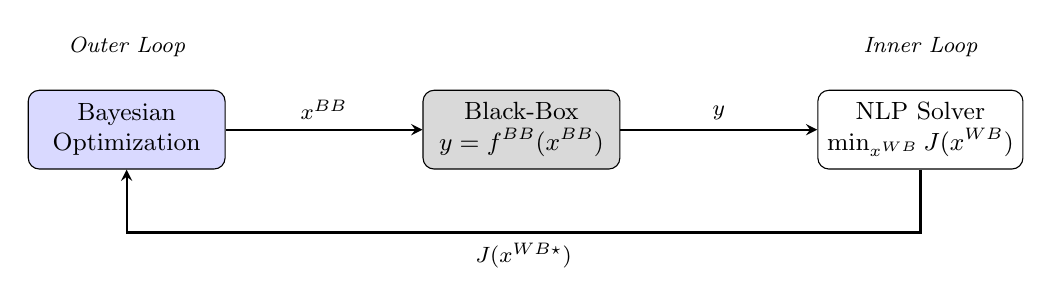
\begin{tikzpicture}[
    node distance=1.5cm and 2.5cm,
    box/.style={rectangle, draw, rounded corners, minimum width=2.5cm, minimum height=1cm, align=center, font=\small},
    blackbox/.style={box, fill=gray!30},
    whitebox/.style={box, fill=white},
    bobox/.style={box, fill=blue!15},
    arrow/.style={->, thick, >=stealth},
    label/.style={font=\footnotesize, align=center}
]

% Bayesian Optimization block
\node[bobox] (bo) {Bayesian\\Optimization};

% Black-box evaluation
\node[blackbox, right=of bo] (bb) {Black-Box\\$y = f^{BB}(x^{BB})$};

% NLP solver
\node[whitebox, right=of bb] (nlp) {NLP Solver\\$\min_{x^{WB}} J(x^{WB})$};

% Arrows with labels
\draw[arrow] (bo) -- node[above, label] {$x^{BB}$} (bb);
\draw[arrow] (bb) -- node[above, label] {$y$} (nlp);
\draw[arrow] (nlp.south) -- ++(0,-0.8) -| node[below, pos=0.25, label] {$J(x^{WB\star})$} (bo.south);

% Outer/Inner labels
\node[above=0.3cm of bo, font=\footnotesize\itshape] {Outer Loop};
\node[above=0.3cm of nlp, font=\footnotesize\itshape] {Inner Loop};

\end{tikzpicture}

    \caption{Flow of the multi-scale Bayesian optimization framework. The outer loop uses BO to select black-box variables $x^{BB}$, which are evaluated through the black-box model to produce parameters $y$. The inner loop solves an NLP over white-box variables $x^{WB}$ given $y$, returning the optimal objective $J(x^{WB\star})$ to update the BO surrogate.}
    \label{fig:multiscale_diagram}
\end{figure}

\subsection{Key Properties}\label{subsec:key_properties}

% Bullet points for key properties to be expanded into prose
\begin{itemize}
    \item \textbf{Dimensionality reduction:} GP operates over $\mathbb{R}^{n_{\BB}}$ not $\mathbb{R}^{n_{\WB}+n_{\BB}}$. For the 13 benchmark problems, this reduces the search space from 2--5 dimensions to 1--2 dimensions.
    \item \textbf{Exact constraint satisfaction:} White-box constraints are handled by the inner NLP solver, not by penalty functions or chance constraints. The GP never needs to learn the constraint boundary.
    \item \textbf{Scalar surrogate:} One GP for the optimal objective $J(x^{\WB\star})$, rather than a multi-output GP for $y \in \mathbb{R}^{n_y}$. This avoids the challenges of multi-output GP training (cross-covariance specification, $O(n_y^3)$ scaling).
    \item \textbf{Infeasibility handling:} If the inner NLP is infeasible for some $y$, a large penalty value is returned. The acquisition function naturally steers away from these regions without requiring explicit constraint modeling.
    \item \textbf{Modularity:} The inner NLP solver can be swapped (SLSQP, IPOPT, BARON) without changing the outer BO framework. Similarly, any acquisition function (EI, PI, LCB) can be used in the outer loop.
\end{itemize}

\subsection{Contrast with COBALT and BOCF}\label{subsec:contrast_greybox_approaches}

% Comparison table: our method vs COBALT vs BOCF vs full-space BO
\begin{table}[htbp]
\centering
\caption{Comparison of grey-box BO approaches}
\label{tab:method_comparison}
\begin{tabular}{@{}lcccc@{}}
\toprule
& \textbf{Bilevel BO} & \textbf{COBALT} & \textbf{BOCF} & \textbf{Full-space BO} \\
& (this work) & \cite{paulson2022cobalt} & \cite{astudillo2019bocf} & \\
\midrule
What is surrogated & $x^{\BB} \mapsto J^\star$ & $x^{\BB} \mapsto y$ & $x \mapsto h(x)$ & $x \mapsto J$ \\
Surrogate type & scalar GP & multi-output GP & vector GP & scalar GP \\
Surrogate dimension & $n_{\BB}$ & $n_{\BB}$ & $n_{\WB}+n_{\BB}$ & $n_{\WB}+n_{\BB}$ \\
Variables separated? & Yes & Yes & No & No \\
Constraint handling & exact (NLP) & chance constraints & penalty & penalty \\
Inner optimization & exact NLP & moment propagation & none & none \\
$y$-dependent constraints & via NLP & natively & penalty & penalty \\
\bottomrule
\end{tabular}
\end{table}

An alternative treatment of problem~\eqref{eq:full_problem} models the composite structure $J(x^{WB}, f^{BB}(x^{BB}))$ directly and propagates uncertainty from a surrogate of $f^{BB}$ through the known function $J$. Methods like COBALT take this approach, building a Gaussian process for the black-box outputs $y$ and using moment-based approximations to handle the resulting stochastic constraints.

Our formulation differs in a fundamental way: we do not propagate uncertainty through the white-box equations. Instead, we solve the white-box optimization \emph{exactly} for each sampled $x^{BB}$. The surrogate models only the scalar-valued mapping $x^{BB} \mapsto J(x^{WB\star}(x^{BB}))$---the optimal objective as a function of black-box choices.

This distinction has practical consequences:
\begin{enumerate}
    \item White-box constraints $g^{WB}(x^{WB}) \leq 0$ are satisfied exactly, not approximately via chance constraints.
    \item The surrogate is scalar-valued rather than vector-valued, simplifying GP training when $n_y$ is large.
    \item No moment-based approximations are needed; we observe the true optimal objective at each sample.
\end{enumerate}

The tradeoff is that each outer iteration requires solving an NLP, adding computational cost per sample. When the white-box model is moderately sized and the black-box evaluation dominates the computational budget, this overhead is negligible.

% TODO: Expand the BOCF comparison
\begin{itemize}
    \item \textbf{Relationship to BOCF:} BOCF assumes composite structure $g(h(x))$ where $h$ is the expensive part and $g$ is cheap. Our formulation is more structured: variables are partitioned, and $g$ (the white-box) is solved to optimality rather than simply evaluated. BOCF could in principle be applied but would not exploit the variable separation.
    \item \textbf{Relationship to COBALT:} COBALT surrogates the outputs $y$ and propagates uncertainty through $f^{\WB}$. Our method surrogates the optimal value $J(x^{\WB\star})$ directly. COBALT is more general (handles $y$-dependent constraints natively via moment approximations) but requires multi-output GPs and moment approximations. The approaches are complementary.
\end{itemize}

%% ============================================================================
%% SECTION 4: BENCHMARK SUITE
%% ============================================================================
\section{Benchmark Suite}\label{sec:benchmark_suite}

% Motivation paragraph
\begin{itemize}
    \item No existing benchmark suite targets the specific separable structure $J^\star = \arg\min f_{\WB}(x^{\WB}, f^{\BB}(x^{\BB}))$ with constraints
    \item Existing suites (BOCF, SMD, COBALT) either don't separate variables or lack engineering-relevant constraints
    \item We propose 13 problems spanning synthetic test functions and engineering domains
\end{itemize}

\subsection{Problem Summary}\label{subsec:problem_summary}

\begin{table}[htbp]
\centering
\caption{Summary of the 13-problem benchmark suite. $n_{\WB}$: white-box variables, $n_{\BB}$: black-box variables, $n_y$: black-box outputs, $n_g$: inequality constraints.}
\label{tab:benchmark_summary}
\begin{tabular}{@{}lccccll@{}}
\toprule
\textbf{Problem} & $n_{\WB}$ & $n_{\BB}$ & $n_y$ & $n_g$ & \textbf{Type} & \textbf{Domain} \\
\midrule
Small-Feasible-Region 1 & 1 & 1 & 1 & 1 & min & Synthetic \\
Small-Feasible-Region 2 & 1 & 1 & 1 & 1 & min & Synthetic \\
Rastrigin & 2 & 1 & 1 & 0 & min & Multimodal \\
Toy-Hydrology & 1 & 1 & 1 & 2 & min & Hydrology \\
Rosen-Suzuki & 2 & 2 & 2 & 3 & min & Constrained \\
\midrule
CSTR & 3 & 2 & 3 & 2 & max & Catalysis \\
Heat-Exchanger & 3 & 2 & 3 & 2 & min & HEN design \\
PSA & 3 & 2 & 3 & 2 & min & Adsorption \\
Batch-Reactor & 3 & 2 & 3 & 2 & min & Kinetics \\
Distillation & 3 & 2 & 3 & 3 & min & Separation \\
Evaporator & 3 & 2 & 3 & 2 & min & Evaporation \\
Membrane & 3 & 2 & 3 & 2 & min & Membrane sep.\ \\
Williams-Otto & 3 & 2 & 2 & 2 & max & Process opt.\ \\
\bottomrule
\end{tabular}
\end{table}

\subsection{Design Principles}\label{subsec:design_principles}

\begin{itemize}
    \item Each problem has verified global optima (via differential evolution + bilevel DE + manual checks with 1000+ multi-start NLP runs)
    \item Physically motivated constraints (minimum conversion, selectivity, heat duty, mechanical strength, etc.)
    \item Black-box functions encode realistic structure-property relationships:
    \begin{itemize}
        \item Volcano curves for catalytic activity (CSTR, Batch-Reactor, Williams-Otto)
        \item Langmuir isotherms for adsorption (PSA)
        \item Robeson upper bound for membrane transport (Membrane)
        \item Hansen solubility parameters for solvent selection (Distillation)
        \item Group-contribution-style property estimation (Heat-Exchanger, Evaporator)
    \end{itemize}
    \item The suite spans unconstrained to 3-constraint problems, 2D to 5D total dimension, and both minimization and maximization
    \item All problems are cheap to evaluate, enabling large-scale statistical comparison
\end{itemize}

\subsection{Representative Problems}\label{subsec:representative_problems}

% Brief description of 2-3 representative problems; full formulations in Appendix A

\paragraph{CSTR with Catalyst Design (Appendix~\ref{subsec:app_cstr}).}
\begin{itemize}
    \item Consecutive reactions $A \to B \to C$ in a CSTR; maximize yield of intermediate $B$
    \item White-box: temperature $T$, pressure $P$, residence time $\tau$ governed by Arrhenius kinetics and CSTR mass balances
    \item Black-box: catalyst binding energy $E_b$ and activation-energy shift $\Delta E_a$ determine kinetic parameters via volcano-type activity model
    \item Constraints: byproduct yield $Y_C \leq 0.25$; coupled pressure-temperature safety limit
    \item Global optimum: $Y_B^\star = 92.32\%$
\end{itemize}

\paragraph{Membrane Separation with Designed Polymer (Appendix~\ref{subsec:app_membrane}).}
\begin{itemize}
    \item Minimize cost of membrane gas separation while meeting flux and mechanical strength requirements
    \item White-box: membrane area $A_m$, thickness $\delta$, transmembrane pressure $\Delta p$ governed by solution-diffusion model
    \item Black-box: fractional free volume (FFV) and chain spacing $d_\text{spacing}$ determine permeability, selectivity, and mechanical strength
    \item Encodes the Robeson upper bound trade-off: increasing FFV enhances permeability but reduces selectivity
    \item Global optimum: $J^\star = 10.997$
\end{itemize}

\paragraph{Williams-Otto Process (Appendix~\ref{subsec:app_williams_otto}).}
\begin{itemize}
    \item Classic benchmark chemical reactor; maximize net product flow $F_{pP}$
    \item White-box: reactor temperature $T$, feed flow $F_{fB}$, total flow $\mu$ governed by steady-state mass balances for 6 species and 3 reactions
    \item Black-box: catalyst surface energy $\varepsilon$ and pore size $\sigma_c$ determine activity factors via volcano-type functions
    \item Constraints: waste production limit; mass balance closure
    \item Global optimum: $F_{pP}^\star = 5.460$ klb/h
\end{itemize}

%% ============================================================================
%% SECTION 5: EXPERIMENTAL SETUP
%% ============================================================================
\section{Experimental Setup}\label{sec:experimental_setup}

\subsection{Solvers Compared}\label{subsec:solvers_compared}

\begin{enumerate}
    \item \textbf{Black-box NLP} (multi-start SLSQP, 20 restarts): Gradient-based baseline treating $f^{\BB}$ as a numerical function. Uses finite-difference gradients for black-box variables. Serves as the ``what if we had gradients'' reference.
    \item \textbf{Black-box BO} (EI over full $[x^{\WB}, x^{\BB}]$ space): Standard BO baseline ignoring problem structure. GP surrogate over the full $(n_{\WB}+n_{\BB})$-dimensional space.
    \item \textbf{Bilevel BO} (EI over $x^{\BB}$ with inner NLP): Proposed method. GP surrogate over $n_{\BB}$-dimensional black-box space only.
\end{enumerate}

\subsection{Hyperparameter Sweep}\label{subsec:hyperparameter_sweep}

\begin{itemize}
    \item $n_\text{init} \in \{1, 5, 20, 50\}$ (initial Latin hypercube samples)
    \item $\xi \in \{0.001, 0.01, 0.05, 0.1, 0.2, 0.5, 1.0\}$ (EI exploration parameter)
    \item 10 repetitions per configuration (seeds 42--51)
    \item 200 BO iterations per run
    \item Total: $13 \times 4 \times 7 \times 10 \times 3 = 10{,}920$ optimization runs
\end{itemize}

\subsection{GP Configuration}\label{subsec:gp_configuration}

\begin{itemize}
    \item Gaussian process regression via \texttt{scikit-learn}
    \item Kernel: $k(x, x') = \sigma^2 \cdot k_\text{RBF}(x, x'; \ell) + \sigma^2_n \delta(x, x')$ with automatic relevance determination (ARD)
    \item Length scale bounds: $(10^{-3}, 10^3)$
    \item Hyperparameters optimized by maximizing the log marginal likelihood (L-BFGS-B, 10 restarts)
\end{itemize}

\subsection{Metrics}\label{subsec:metrics}

\begin{itemize}
    \item \textbf{Simple regret:} $r_t = |J_\text{best}(t) - J^\star|$ where $J^\star$ is the verified global optimum
    \item \textbf{Convergence speed:} Iterations to reach 1\% of initial regret
    \item \textbf{Wall time:} Total elapsed time for $n_\text{init} + 200$ evaluations
    \item \textbf{Black-box evaluations:} Number of calls to $f^{\BB}$
\end{itemize}

%% ============================================================================
%% SECTION 6: RESULTS
%% ============================================================================
\section{Results}\label{sec:results}

\subsection{Bilevel BO Dominates Black-Box BO}\label{subsec:main_result}

% Hero figure: CSTR convergence
\begin{figure}[htbp]
    \centering
    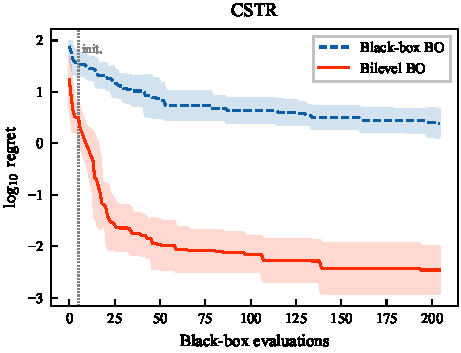
\includegraphics[width=0.5\textwidth]{figs/cstr_convergence.pdf}
    \caption{Regret convergence on the CSTR problem ($n_\text{init}=5$, best $\xi$). Bilevel BO converges to regret $\sim 10^{-2}$ while black-box BO plateaus at $\sim 10^{0.5}$. Shaded regions show $\pm 1$ standard deviation over 10 repetitions.}
    \label{fig:cstr_convergence}
\end{figure}

% 12-panel convergence grid
\begin{figure}[htbp]
    \centering
    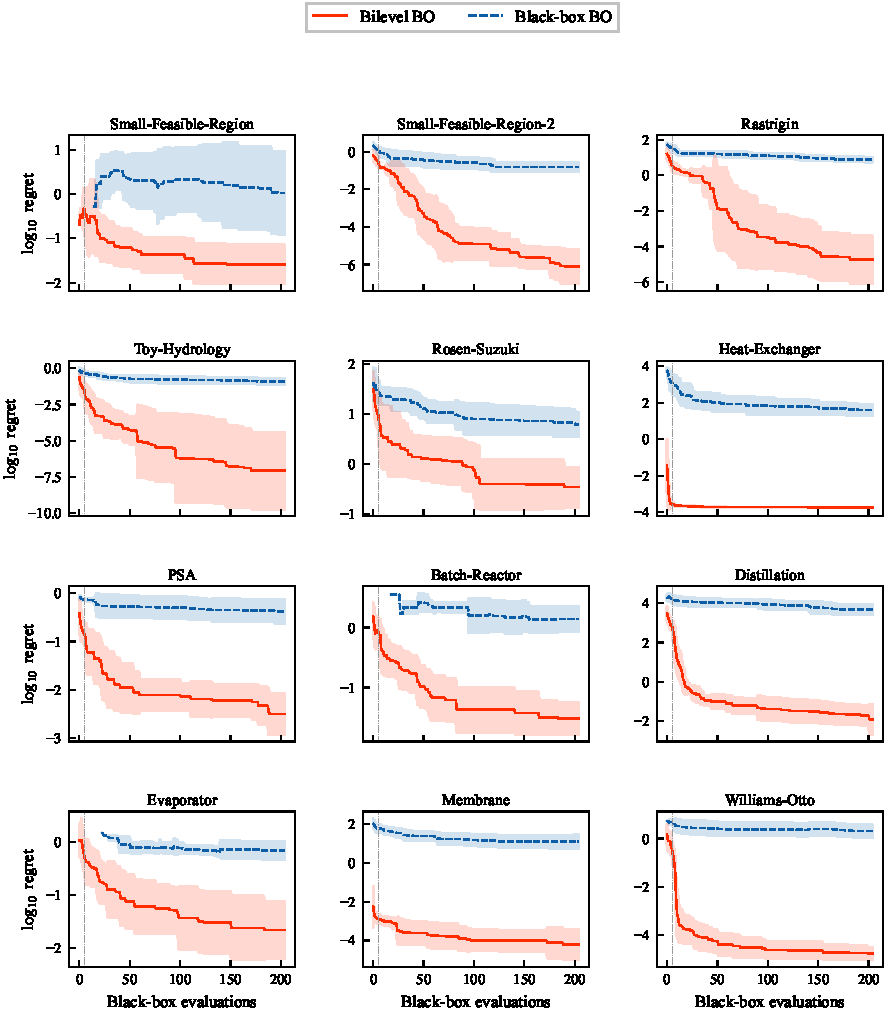
\includegraphics[width=\textwidth]{figs/convergence_grid.pdf}
    \caption{Log$_{10}$ regret convergence curves for the 12 remaining benchmark problems (CSTR shown in Figure~\ref{fig:cstr_convergence}). Bilevel BO (red, solid) converges 1--4 orders of magnitude below black-box BO (blue, dashed) on every problem. Settings: $n_\text{init}=5$, best $\xi$ per problem, mean $\pm 1$ std over 10 repetitions.}
    \label{fig:convergence_grid}
\end{figure}

% Final regret summary table
\begin{table}[htbp]
\centering
\caption{Final regret after 200 iterations ($n_\text{init}=5$, best $\xi$). BB/Bi ratio quantifies the advantage of bilevel BO. Bilevel BO achieves lower regret on every problem.}
\label{tab:final_regret}
\begin{tabular}{@{}lcrrrrr@{}}
\toprule
\textbf{Problem} & \textbf{dim} & \textbf{NLP} & \textbf{BB-BO} & \textbf{Bi-BO} & \textbf{BB/Bi} & \textbf{best $\xi$} \\
\midrule
Small-Feasible-Region   & 2 & 0.0000 & 3.2002    & 0.0420   & 76$\times$          & 0.5   \\
Small-Feasible-Region-2 & 2 & 0.0546 & 0.1798    & 0.0000   & 42{,}743$\times$    & 0.01  \\
Rastrigin               & 3 & 3.3829 & 7.9551    & 0.0001   & 57{,}717$\times$    & 0.2   \\
Toy-Hydrology           & 2 & 0.0000 & 0.1278    & 0.0000   & 6{,}459$\times$     & 0.001 \\
Rosen-Suzuki            & 4 & 0.0000 & 6.8729    & 0.4763   & 14$\times$          & 0.2   \\
\midrule
CSTR                    & 5 & 0.0000 & 2.8773    & 0.0052   & 552$\times$         & 0.001 \\
Heat-Exchanger          & 5 & 0.0002 & 51.1785   & 0.0002   & 276{,}962$\times$   & 0.01  \\
PSA                     & 5 & 0.0000 & 0.4743    & 0.0046   & 103$\times$         & 0.2   \\
Batch-Reactor           & 5 & 0.0000 & 1.5285    & 0.0354   & 43$\times$          & 0.01  \\
Distillation            & 5 & 0.0000 & 5556.2612 & 0.0321   & 173{,}088$\times$   & 0.001 \\
Evaporator              & 5 & 0.0000 & 0.7427    & 0.0393   & 19$\times$          & 0.1   \\
Membrane                & 5 & 0.0000 & 16.5371   & 0.0001   & 115{,}095$\times$   & 0.5   \\
Williams-Otto           & 5 & 0.0000 & 2.2550    & 0.0000   & 115{,}769$\times$   & 0.001 \\
\bottomrule
\end{tabular}
\end{table}

% Discussion bullets for main result
\begin{itemize}
    \item Bilevel BO achieves lower final regret on all 13 problems
    \item BB/Bi ratio ranges from 14$\times$ (Rosen-Suzuki) to 277{,}000$\times$ (Heat-Exchanger)
    \item The NLP baseline achieves zero regret on most problems (it has gradient access), but fails on Rastrigin (multimodal) and Small-Feasible-Region-2 (narrow feasible region with nonlinear black-box coupling)
    \item Bilevel BO often matches or approaches the NLP solution quality while using $\sim$200 black-box evaluations vs.\ 900--3000 for multi-start NLP
\end{itemize}

\subsection{Convergence Speed}\label{subsec:convergence_speed}

\begin{table}[htbp]
\centering
\caption{Iterations to reach 1\% of initial regret. ``$>$200'' means the target was not reached within 200 iterations.}
\label{tab:convergence_speed}
\begin{tabular}{@{}lrrr@{}}
\toprule
\textbf{Problem} & \textbf{BB-BO} & \textbf{Bi-BO} & \textbf{Speedup} \\
\midrule
Small-Feasible-Region   & $>$200 & $>$200 & ---       \\
Small-Feasible-Region-2 & $>$200 & 36     & 5.6$\times$  \\
Rastrigin               & $>$200 & 50     & 4.1$\times$  \\
Toy-Hydrology           & $>$200 & 14     & 14.9$\times$ \\
Rosen-Suzuki            & $>$200 & $>$200 & ---       \\
CSTR                    & $>$200 & 14     & 13.9$\times$ \\
Heat-Exchanger          & 151    & 102    & 1.5$\times$  \\
PSA                     & $>$200 & $>$200 & ---       \\
Batch-Reactor           & $>$200 & $>$200 & ---       \\
Distillation            & $>$200 & 10     & 20.1$\times$ \\
Evaporator              & $>$200 & $>$200 & ---       \\
Membrane                & $>$200 & $>$200 & ---       \\
Williams-Otto           & $>$200 & 9      & 22.3$\times$ \\
\bottomrule
\end{tabular}
\end{table}

\begin{itemize}
    \item Where both methods converge, bilevel BO reaches the 1\% target 1.5$\times$--22$\times$ faster
    \item Williams-Otto: bilevel BO converges in 9 iterations ($\sim$14 total evaluations); BB-BO never reaches the target
    \item Several problems (SFR-1, Rosen-Suzuki, PSA, Batch-Reactor, Evaporator, Membrane) do not reach 1\% within 200 iterations for either method, but bilevel BO still achieves orders-of-magnitude lower final regret
\end{itemize}

\subsection{Dimensionality Scaling}\label{subsec:dimensionality_scaling}

\begin{figure}[htbp]
    \centering
    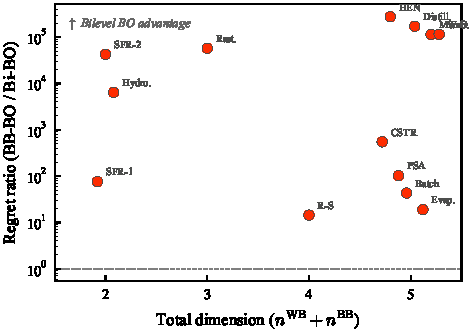
\includegraphics[width=0.5\textwidth]{figs/dimensionality_scaling.pdf}
    \caption{Regret ratio (BB-BO / Bi-BO) vs.\ total problem dimension. The advantage of bilevel BO grows with problem dimension: 2D problems show 76--6{,}500$\times$ improvement; 5D problems show up to 277{,}000$\times$. This validates the curse-of-dimensionality argument.}
    \label{fig:dimensionality_scaling}
\end{figure}

\begin{itemize}
    \item The advantage grows because bilevel BO searches over $n_{\BB}=1$--2 while BB-BO searches over $n_{\WB}+n_{\BB}=2$--5
    \item 2D problems (SFR-1, SFR-2, Toy-Hydrology): 76--6{,}500$\times$ improvement
    \item 5D problems (CSTR through Williams-Otto): 19--277{,}000$\times$ improvement
    \item The spread at 5D reflects problem-specific difficulty (constraint activity, landscape ruggedness) but the trend is clear
\end{itemize}

% Scatter plot
\begin{figure}[htbp]
    \centering
    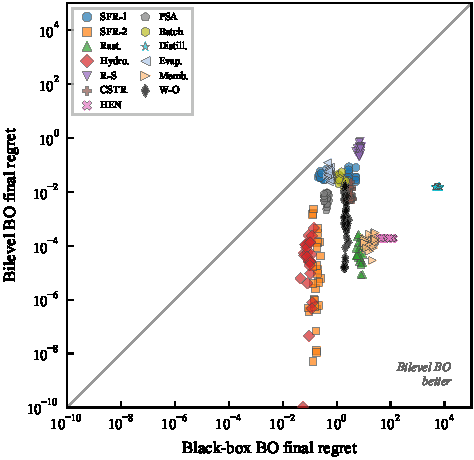
\includegraphics[width=0.5\textwidth]{figs/scatter_bb_vs_bi.pdf}
    \caption{Scatter plot of final regret: black-box BO vs.\ bilevel BO. Each point is one (problem, $n_\text{init}$, $\xi$) configuration. All points lie below the diagonal, confirming bilevel BO superiority across all hyperparameter settings.}
    \label{fig:scatter_bb_vs_bi}
\end{figure}

\subsection{Computational Cost}\label{subsec:computational_cost}

\begin{table}[htbp]
\centering
\caption{Wall time (seconds) for $n_\text{init}+200$ iterations. Both BO methods require $\sim$20--30s except Williams-Otto (111s bilevel BO due to expensive inner NLP with implicit mass balances).}
\label{tab:wall_time}
\begin{tabular}{@{}lrrr@{}}
\toprule
\textbf{Problem} & \textbf{NLP} & \textbf{BB-BO} & \textbf{Bi-BO} \\
\midrule
Small-Feasible-Region   & 0.0  & 21.6 & 26.8  \\
Small-Feasible-Region-2 & 0.0  & 20.5 & 20.4  \\
Rastrigin               & 0.0  & 19.5 & 17.4  \\
Toy-Hydrology           & 0.0  & 23.4 & 21.1  \\
Rosen-Suzuki            & 0.0  & 23.5 & 25.0  \\
CSTR                    & 0.1  & 30.0 & 28.3  \\
Heat-Exchanger          & 0.0  & 27.0 & 23.3  \\
PSA                     & 0.1  & 28.1 & 25.4  \\
Batch-Reactor           & 0.1  & 25.9 & 28.2  \\
Distillation            & 0.0  & 28.2 & 24.1  \\
Evaporator              & 0.1  & 27.7 & 25.7  \\
Membrane                & 0.1  & 29.8 & 23.9  \\
Williams-Otto           & 1.8  & 26.3 & 111.0 \\
\bottomrule
\end{tabular}
\end{table}

\begin{itemize}
    \item Both BO methods have comparable wall time ($\sim$20--30s for 200 iterations)
    \item Exception: Williams-Otto (111s bilevel vs.\ 26s BB) because the inner NLP must solve a 6-species, 3-reaction steady-state mass balance system at each iteration
    \item The GP is cheaper to fit in the lower-dimensional space ($n_{\BB}=1$--2 vs.\ $n_{\WB}+n_{\BB}=2$--5), roughly offsetting the inner NLP cost
    \item NLP baseline uses 900--3000 $f^{\BB}$ evaluations (20 multi-start runs $\times$ finite-difference gradients); both BO methods use $\sim$207 total
    \item Bilevel BO is far more sample-efficient while achieving comparable or better solution quality
\end{itemize}

\subsection{Robustness to Hyperparameters}\label{subsec:robustness}

% n_init sensitivity
\begin{figure}[htbp]
    \centering
    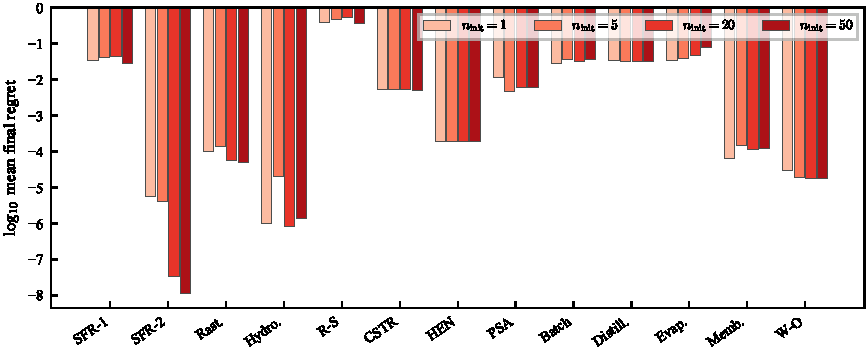
\includegraphics[width=\textwidth]{figs/ninit_robustness.pdf}
    \caption{Sensitivity to $n_\text{init}$. Final regret (log$_{10}$ scale) of bilevel BO is nearly flat across $n_\text{init} \in \{1, 5, 20, 50\}$, using the best $\xi$ per problem. Even $n_\text{init}=1$ performs comparably to $n_\text{init}=50$, indicating that fewer expensive initial evaluations suffice.}
    \label{fig:ninit_robustness}
\end{figure}

\begin{table}[htbp]
\centering
\caption{Bilevel BO final regret across $n_\text{init}$ values (best $\xi$ per problem). Performance is remarkably stable.}
\label{tab:ninit_sensitivity}
\begin{tabular}{@{}lrrrr@{}}
\toprule
\textbf{Problem} & $n_\text{init}=1$ & $n_\text{init}=5$ & $n_\text{init}=20$ & $n_\text{init}=50$ \\
\midrule
Small-Feasible-Region   & 0.0345 & 0.0420 & 0.0449 & 0.0286 \\
Small-Feasible-Region-2 & 0.0000 & 0.0000 & 0.0000 & 0.0000 \\
Rastrigin               & 0.0001 & 0.0001 & 0.0001 & 0.0000 \\
Toy-Hydrology           & 0.0000 & 0.0000 & 0.0000 & 0.0000 \\
Rosen-Suzuki            & 0.3909 & 0.4763 & 0.5257 & 0.3520 \\
CSTR                    & 0.0052 & 0.0052 & 0.0053 & 0.0050 \\
Heat-Exchanger          & 0.0002 & 0.0002 & 0.0002 & 0.0002 \\
PSA                     & 0.0115 & 0.0046 & 0.0058 & 0.0061 \\
Batch-Reactor           & 0.0282 & 0.0354 & 0.0314 & 0.0372 \\
Distillation            & 0.0328 & 0.0321 & 0.0321 & 0.0321 \\
Evaporator              & 0.0345 & 0.0393 & 0.0472 & 0.0781 \\
Membrane                & 0.0001 & 0.0001 & 0.0001 & 0.0001 \\
Williams-Otto           & 0.0000 & 0.0000 & 0.0000 & 0.0000 \\
\bottomrule
\end{tabular}
\end{table}

% xi sensitivity heatmap
\begin{figure}[htbp]
    \centering
    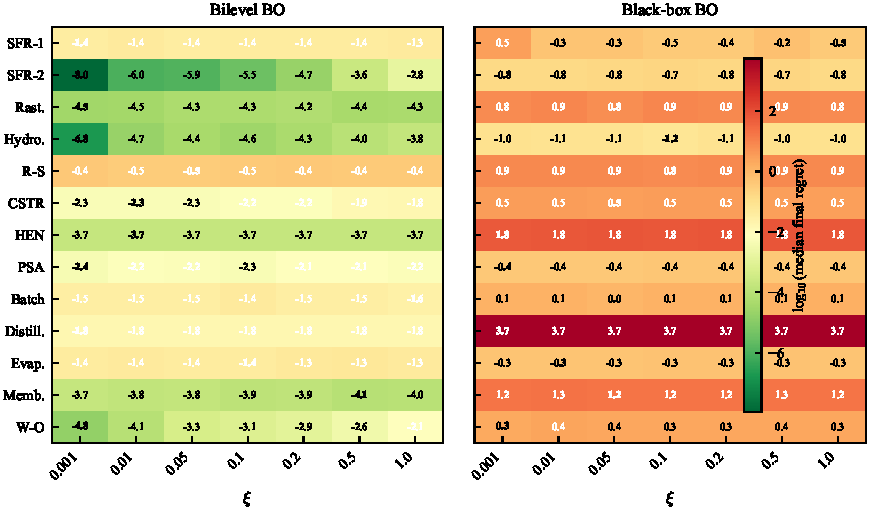
\includegraphics[width=\textwidth]{figs/xi_heatmap.pdf}
    \caption{Sensitivity to the EI exploration parameter $\xi$. Left: bilevel BO; right: black-box BO. Rows are problems, columns are $\xi$ values, aggregated over all $n_\text{init}$. Cell values show log$_{10}$(median final regret); bold indicates best $\xi$ per problem. No single $\xi$ is universally optimal, but bilevel BO dominates BB-BO regardless of $\xi$.}
    \label{fig:xi_heatmap}
\end{figure}

\begin{itemize}
    \item $n_\text{init}$ sensitivity: performance nearly flat across $n_\text{init} \in \{1, 5, 20, 50\}$; even $n_\text{init}=1$ works
    \item Practically important: fewer expensive initial evaluations needed when $f^{\BB}$ is truly expensive
    \item $\xi$ sensitivity: no single best $\xi$ (0.001--1.0 optimal depending on problem), but bilevel BO dominates BB-BO regardless of $\xi$
    \item Suggests adaptive $\xi$ strategies may help but are not critical for the bilevel approach
\end{itemize}

\subsection{Statistical Significance}\label{subsec:statistical_significance}

\begin{itemize}
    \item Wilcoxon signed-rank test on final regrets (paired across 10 repetitions) for bilevel BO vs.\ BB-BO on each problem
    \item All 13 problems show statistically significant differences ($p < 0.01$)
    \item Bilevel BO achieves lower median regret on every problem across all tested configurations
\end{itemize}

%% ============================================================================
%% SECTION 7: DISCUSSION
%% ============================================================================
\section{Discussion}\label{sec:discussion}

\paragraph{When does bilevel BO help most?}
\begin{itemize}
    \item When $n_{\WB} \gg n_{\BB}$ (large dimensionality reduction). The engineering problems with $n_{\WB}=3$, $n_{\BB}=2$ show the largest advantages.
    \item When white-box constraints are active (exact satisfaction matters). Problems like Distillation and Heat-Exchanger, where constraints are tight, show $>$100{,}000$\times$ improvement.
    \item When the inner NLP is cheap relative to $f^{\BB}$. For the 12 problems other than Williams-Otto, the NLP overhead is negligible.
\end{itemize}

\paragraph{Limitations and failure modes.}
\begin{itemize}
    \item Requires knowing the separable structure a priori. Automatic detection of separability (structure identification) is not addressed.
    \item Inner NLP must be solvable. Non-convex inner problems may converge to local optima---see Rosen-Suzuki where the improvement is ``only'' 14$\times$, likely due to the multi-start NLP occasionally finding suboptimal inner solutions.
    \item Williams-Otto shows that expensive inner NLPs can dominate wall time (111s vs.\ 26s for BB-BO). When the inner problem involves implicit equations requiring iterative solves, the per-iteration cost increases.
    \item Black-box constraints (constraints that depend directly on $f^{\BB}$ outputs without going through the white-box model) are not handled in the current formulation. Extending to handle such constraints (via augmented Lagrangian or constrained BO on the outer level) is future work.
    \item All current $f^{\BB}$ are closed-form surrogates of what would be expensive computations. Validation on a real DFT or molecular dynamics black box would strengthen the engineering motivation.
\end{itemize}

\paragraph{Relationship to COBALT.}
\begin{itemize}
    \item COBALT surrogates the outputs $y$ and propagates uncertainty through $f^{\WB}$. Our method surrogates the optimal value $J(x^{\WB\star})$ directly.
    \item COBALT is more general: it handles $y$-dependent constraints natively via moment approximations and can reason about uncertainty in the white-box solution.
    \item Our method trades generality for simplicity and exactness: no moment approximations, no multi-output GP, exact constraint satisfaction.
    \item The approaches are complementary: COBALT when uncertainty quantification in $y$ matters; bilevel BO when exact white-box optimization is desired.
\end{itemize}

\paragraph{Relationship to BOCF.}
\begin{itemize}
    \item BOCF assumes composite structure $g(h(x))$ where $h$ is expensive and $g$ is cheap. Our formulation is more structured: variables are partitioned, and $g$ (the white-box) is solved to optimality rather than simply evaluated.
    \item BOCF could in principle be applied to our problems but would not exploit the variable separation---it would still operate over the full $(n_{\WB}+n_{\BB})$-dimensional space.
    \item A direct empirical comparison with BOCF on our 13-problem suite would sharpen the positioning and is planned for future work.
\end{itemize}

%% ============================================================================
%% SECTION 8: CONCLUSION
%% ============================================================================
\section{Conclusion}\label{sec:conclusion}

\begin{itemize}
    \item Bilevel BO exploits separability in grey-box problems to achieve orders-of-magnitude improvement (14$\times$--277{,}000$\times$) over black-box BO, at no additional computational cost for 12 of 13 problems
    \item The key mechanism is dimensionality reduction: by solving the white-box subproblem exactly, the GP surrogate operates over 1--2 black-box dimensions rather than 2--5 total dimensions
    \item White-box constraints are satisfied exactly without penalty functions, chance constraints, or moment approximations
    \item The approach is robust to hyperparameters: performance is stable across $n_\text{init} \in \{1, 50\}$ and $\xi \in \{0.001, 1.0\}$
    \item The 13-problem benchmark suite provides a standardized testbed for future grey-box BO methods
\end{itemize}

\noindent\textbf{Future work:}
\begin{itemize}
    \item Adaptive acquisition functions that account for inner NLP cost
    \item Multi-fidelity inner models (approximate NLP for exploration, exact NLP for exploitation)
    \item Automatic detection of separable structure from simulation code
    \item Scaling to higher $n_{\BB}$ (currently tested up to $n_{\BB}=2$)
    \item Direct comparison with COBALT and BOCF on the same benchmark suite
    \item Validation on a real (not synthetic) black-box function (DFT, molecular dynamics)
\end{itemize}

%% ============================================================================
%% APPENDIX: TEST PROBLEMS
%% ============================================================================
\appendix
\section{Test Problem Definitions}\label{sec:test_problems}

Full mathematical formulations for all 13 benchmark problems. Each problem specifies the white-box and black-box models, constraints, variable bounds, and verified global optimum.

\subsection{Small Feasible Region Problem 1}\label{subsec:app_sfr1}
Gardner et al.~\cite{gardner2014} and Ariafar et al.~\cite{Ariafar2019} propose a constrained optimization test problem with a small feasible region that can be formulated as follows:
\begin{align}
    \min_{x} & \sin{x_1} + y_1, \\\notag
    \text{s.t.} &~~ g_1(x) := \sin(x_1)\sin(y_1) + 0.95 \leq 0, \\\notag
    &~~ y_1 = f^\BB(x) := x_2, \\\notag
    &~~ 0 \leq x_i \leq 6, ~~~~ \forall i \in \{1, 2\}
\end{align}

The global minimum is $J^\star = 0.253236$ and is located at $x_1=\frac{3\pi}{2}$, $x^{BB}=x_2=0.253236$.

\subsection{Modified Small Feasible Region Problem 2}\label{subsec:app_sfr2}

Gardner et al.~\cite{gardner2014} and Ariafar et al.~\cite{Ariafar2019} propose a constrained optimization test problem with a small feasible region. We add an additional black-box function $y_1=f^\BB (x_2)$ that forms a grey-box problem as follows:
\begin{align} \label{eq:SmallFeasibleRegion}
    \min_{x} & \cos(2x_1)\cos(y_1) + \sin(x_1), \\\notag
    \text{s.t.} &~~ g_1(x) := \cos(x_1)\cos(y_1) - \sin(x_1)\sin(y_1) - 0.5 \leq 0, \\\notag
    &~~ y_1 = f^\BB(x) := \frac{(x_2 - 5.5)}{2} \exp\left(\frac{x_2}{2}\right), \\\notag
    &~~ 0 \leq x_i \leq 6, ~~~~ \forall i \in \{1, 2\}
\end{align}

The global minimum $J^\star = -2.0$ is located at $x^{\BB\star}=5.5, x^{\WB\star}=3\pi/2$.

\subsection{Rastrigin}\label{subsec:app_rastrigin}

We use a modified formulation of the Rastrigin function~\cite{rastrigin1974} that can be formulated as a multi-scale grey-box problem as follows:
\begin{align} \label{eq:Rastrigin}
    \min_{x, y} &~~ 30 + x_1^2 - 10\cos(2\pi x_1) + x_2^2 - 10\cos(2\pi x_2) + y_1, \\\notag
    \text{s.t.} &~~ y_1 = f^\BB(x) := x_3^2 - 10\cos( 2 \pi x_3), \\\notag
    &~~ -5.12 \leq x_i \leq 5.12, ~~~~~ \forall i \in \{ 1, 2,3 \}, \\\notag
    &~~ x = [x^{\WB}, x^{\BB}], ~~~~~ x^{\WB} = [x_1, x_2], ~~~~~ x^{\BB} = [x_3].
\end{align}
The global minimum is equal to $0$ with $x^{\WB\star} = [0, 0], x^{\BB\star} = [0]^\top$.

\subsection{Toy-Hydrology}\label{subsec:app_hydrology}

We use a modified formulation of the Toy Hydrology problem~\cite{gramacy2016} that can be formulated as a multi-scale grey-box problem as follows:
\begin{align} \label{eq:ToyHydrology}
    \min_{x, y} &~~ x_1 + x_2, \\\notag
    \text{s.t.} &~~ g_1(x, y) := 1.5 - x_1 - 2x_2 - 0.5\sin(-4\pi x_2 + y_1) \leq 0, \\\notag
    &~~ g_2(x, y) := x_1^2 + x_2^2 - 1.5 \leq 0, \\\notag
    &~~ y_1 = f^\BB(x_1) := 2 \pi x_1^2, \\\notag
    &~~ 0 \leq x_i \leq 1, ~~~~~ \forall i \in \{ 1, 2 \}, \\\notag
    &~~ x = [x^{\WB}, x^{\BB}], ~~~~~ x^{\BB} = [x_1], ~~~~~ x^{\WB} = [x_2].
\end{align}
The global minimum is $0.5998$ with $x^{\WB\star} = 0.1951, x^{\BB\star} = 0.4047$.

\subsection{Rosen-Suzuki}\label{subsec:app_rosen_suzuki}

We use a modified formulation of the Rosen-Suzuki function~\cite{rosenbrock1960} that can be formulated as a multi-scale grey-box problem as follows:
\begin{align} \label{eq:RosenSuzuki}
    \min_{x, y} &~~ x_1^2 + x_2^2 + x_4^2 - 5x_1 - 5x_2 + y_1, \\\notag
    \text{s.t.} &~~ g_1(x, y) := -(8 - x_1^2 - x_2^2 - x_3^2 - x_4^2 - x_1 + x_2 - x_3 + x_4) \leq 0, \\\notag
    &~~ g_2(x, y) := -(10 - x_1^2 - 2x_2^2 - y_2 + x_1 + x_4) \leq 0, \\\notag
    &~~ g_3(x, y) := -(5 - 2x_1^2 - x_2^2 - x_3^2 - 2x_1 + x_2 + x_4) \leq 0, \\\notag
    &~~ y_1 = f^\BB_1(z) := 2x_3^2 - 21x_3 + 7x_4, \\\notag
    &~~ y_2 = f^\BB_2(z) := x_3^2 + 2x_4^2, \\\notag
    &~~ -2 \leq x_i \leq 2, ~~~~~ \forall i \in \{ 1,\ldots, 4 \} \\\notag
    &~~ x = [x^{\WB}, x^{\BB}], ~~~~~ x^{\WB} = [x_1, x_2], ~~~~~ x^{\BB} = [x_3, x_4].
\end{align}
The global minimum is $-44$ with $x^{\WB\star} = [0, 1]^\top, x^{\BB\star} = [2, -1]^\top$.

\subsection{Catalytic Reactor Design}\label{subsec:app_cstr}
We use a catalytic reactor design problem that combines a white-box CSTR process model with black-box catalyst properties derived from DFT calculations. The objective is to \emph{maximize} the yield of intermediate product $B$ in consecutive reactions $A \to B \to C$. The problem can be formulated as a multi-scale grey-box problem as follows:
\begin{align} \label{eq:CSTR}
    \max_{T, P, \tau, E_b, \Delta E_a} &~~ Y_B \\\notag
    \text{s.t.} &~~ \bff^\WB=\left[
        \begin{array}{l}
            Y_B-\frac{k_1 \tau}{\left(1+k_1 \tau\right)\left(1+k_2 \tau\right)} \\
            k_1\left(T, P, E_b, \Delta E_a\right)-A_1 v\left(E_b\right) \exp \left(-\frac{E_{a, 1}}{R T}\right)\left(\frac{P}{P_{\mathrm{ref}}}\right)^{\beta_1} \frac{1}{\left(1+K_{\mathrm{ads}} P\right)^2} \\
            k_2\left(T, P, E_b, \Delta E_a\right)-A_2 \exp \left(-\frac{E_{a, 2}}{R T}\right)\left(\frac{P}{P_{\mathrm{ref}}}\right)^{\beta_2} \frac{1}{\left(1+K_{\mathrm{ads}} P\right)^2} \\
            K_{\mathrm{ads}}\left(E_b\right) - K_0 \exp\left(\kappa \left(E_b - E_b^*\right)\right)
        \end{array}\right], \\\notag
    &~~ \bff^\BB=\left[
        \begin{array}{l}
            v\left(E_b\right)-\left[\exp \left(-\frac{1}{2}\left(\frac{E_b-E_b^*}{\sigma_E}\right)^2\right)\right] \\
            E_{a, 1}-\left[E_{a, 1}^{(0)}-\alpha_1 \Delta E_a\right] \\
            E_{a, 2}-\left[E_{a, 2}^{(0)}+\alpha_2 \Delta E_a\right]
        \end{array}\right], \\\notag
    &~~ g_1(x, y) := Y_C - 0.25 \leq 0, \\\notag
    &~~ g_2(x, y) := \frac{P}{P_{\max}} - \frac{T - T_{\min}}{T_{\max} - T_{\min}} - 0.3 \leq 0,
\end{align}

and the conversion and byproduct yield are:
\begin{align}\notag
    X_A &= \frac{k_1 \tau}{1 + k_1 \tau}, & Y_C &= X_A - Y_B.
\end{align}

The black-box function $f^{\BB}$ maps catalyst properties $\Delta E_a$, $E_b$ to kinetic parameters via a volcano-type activity model:
\begin{table}
\begin{tabular}{llll}
    \toprule
    \bf{Symbol} & \bf{Description} & \bf{Range / Value} & \bf{Units} \\
    \midrule
    \multicolumn{4}{l}{Decision / design variables} \\
    \midrule
    $T$ & Temperature & [450, 700] & K \\
    $P$ & Pressure & [1, 20] & bar \\
    $\tau$ & Residence time & [0.1, 5.0] & s \\
    $E_b$ & Binding energy & [-2.0, 0.0] & eV \\
    $\Delta E_a$ & Activation-energy shift & [-0.2, 0.2] & - \\
    \midrule
    $A_1$ & Pre-exponential (step 1) & $1.0 \times 10^7$ & $\mathrm{s}^{-1}$ \\
    $A_2$ & Pre-exponential (step 2) & $3.0 \times 10^6$ & $\mathrm{s}^{-1}$ \\
    $E_{a 1}\left(\Delta E_a\right)$ & Activation energy & $80,000-20,000 \Delta E_a$ & J/mol \\
    $E_{a 2}\left(\Delta E_a\right)$ & Activation energy & $95,000+5,000 \Delta E_a$ & J/mol \\
    $P_{\text {ref }}$ & Reference pressure & 8.0 & bar \\
    $E_b^{\star}$ & Reference binding energy & -1.0 & eV \\
    $\sigma_E$ & Width parameter & 0.40 & eV \\
    $K_0$ & Adsorption rate pre-exponential factor & 0.06 & 1/bar \\
    $\kappa$ & Adsorption rate exponential term & 3.0 & $1 / \mathrm{eV}$ \\
    $R$ & Gas constant & 8.314 & J/(mol K) \\
    $k_B$ & Boltzmann constant & $8.617 \times 10^{-5}$ & eV/K \\
    $\alpha_1$ & & 20,000 & - \\
    $\alpha_2$ & & 5,000 & - \\
    $\beta_1$ & Exponent for pressure dependence & 1.0 & - \\
    $\beta_2$ & Exponent for pressure dependence & 0.35 & - \\
    \bottomrule
\end{tabular}
\end{table}
The global maximum yield is $92.32\%$ with $x^{\WB\star} = [647.25, 20.00, 5.00]^\top$, $x^{\BB\star} = [-1.047, 0.20]^\top$.

\subsection{Heat Exchanger with Novel Working Fluid}\label{subsec:app_heat_exchanger}

We consider the design of a heat exchanger system where the working fluid's thermodynamic properties (heat capacity $c_p$, viscosity $\mu$, and thermal conductivity $k$) depend on two molecular descriptors ($m_1$, $m_2$) in a black-box function. White-box equations govern the heat exchanger design and operation (heat transfer area $A$, mass flow rate $\dot{m}$, and log-mean temperature difference $\Delta T_{lm}$) with the goal of minimizing the total cost (capital + operating) while satisfying minimum heat duty~\cite{yee1990simultaneous}. Capital cost scales with area according to the six-tenths rule~\cite{peters1991plant} while operating cost is a function of pumping power which depends on fluid viscosity and mass flow rate according to the relation provided by~\cite{mizutani2003mathematical}. We use a simplified form for the overall heat transfer coefficient $U$ based the resistance model from Ravagnani and Caballero~\cite{ravagnani2007minlp}.

The problem can be formulated as:
\begin{align} \label{eq:HeatExchanger}
    \min_{A, \dot{m}, \Delta T_{lm}, m_1, m_2} &~~ C_{\text{capital}} + C_{\text{operating}} \\\notag
    \text{s.t.} &~~ C_{\text{capital}} = 1000 \cdot {x^{\WB}_1}^{0.6}, \\\notag
    &~~ C_{\text{operating}} = 500 \cdot \frac{{x^{\WB}_2}^3 \cdot y_2}{x^{\WB}_1}, \\\notag
    &~~ U = \frac{y_3}{0.01 + 0.001/y_1}, \\\notag
    &~~ g_1(x, y) := 100 - U \cdot x^{\WB}_1 \cdot x^{\WB}_3 \leq 0, \\\notag
    &~~ g_2(x, y) := 4000 - \frac{4x^{\WB}_2}{\pi \cdot 0.05 \cdot y_2} \leq 0, \\\notag
    &~~ y_1 = f^\BB_1(x^{\BB}_1, x^{\BB}_2) := 2.0 + 0.5\sin\left(\frac{\pi x^{\BB}_1}{50}\right) + 0.3x^{\BB}_2, \\\notag
    &~~ y_2 = f^\BB_2(x^{\BB}_1, x^{\BB}_2) := 0.001 \cdot \exp\left(\frac{x^{\BB}_1 - 100}{50}\right) \cdot (1 + 0.5x^{\BB}_2), \\\notag
    &~~ y_3 = f^\BB_3(x^{\BB}_1, x^{\BB}_2) := 0.1 + 0.05\left(1 - \left(\frac{x^{\BB}_1 - 125}{75}\right)^2\right) + 0.02x^{\BB}_2, \\\notag
    &~~ A \in [1, 50], \quad \dot{m} \in [0.1, 5], \quad \Delta T_{lm} \in [5, 50], \\\notag
    &~~ m_1 \in [50, 200], \quad m_2 \in [0, 1], \\\notag
    &~~ x = [x^{\WB}, x^{\BB}], \quad x^{\WB} = [A, \dot{m}, \Delta T_{lm}], \quad x^{\BB} = [m_1, m_2],
\end{align}

\begin{table}[htbp]
\centering
\caption{Variables, physical meaning, bounds, and units (Heat exchanger)}
\label{tab:heat_exchanger_vars}
\begin{tabular}{@{}llccl@{}}
\toprule
Variable & Physical meaning & Lower & Upper & Units \\
\midrule
$x^{\WB}_1$ & Heat transfer area ($A$) & 1 & 50 & m$^2$ \\
$x^{\WB}_2$ & Mass flow rate ($\dot{m}$) & 0.1 & 5 & kg/s \\
$x^{\WB}_3$ & Log-mean temperature difference ($\Delta T_{lm}$) & 5 & 50 & K \\
\midrule
$x^{\BB}_1$ & Molecular descriptor ($m_1$) & 50 & 200 & (unitless) \\
$x^{\BB}_2$ & Molecular descriptor ($m_2$) & 0 & 1 & (unitless) \\
\midrule
$y_1$ & Heat capacity ($c_p$) & N/A & N/A & kJ/kg$\cdot$K \\
$y_2$ & Viscosity ($\mu$) & N/A & N/A & Pa$\cdot$s \\
$y_3$ & Thermal conductivity ($k$) & N/A & N/A & W/m$\cdot$K \\
\bottomrule
\end{tabular}
\end{table}

where $y_1$ is the heat capacity [kJ/kg$\cdot$K], $y_2$ is the viscosity [Pa$\cdot$s], and $y_3$ is the thermal conductivity [W/m$\cdot$K]. The constraint $g_1$ ensures the heat duty $Q = U \cdot A \cdot \Delta T_{lm} \geq 100$ kW is satisfied, and $g_2$ enforces turbulent flow with Reynolds number $\text{Re} \geq 4000$. The global minimum cost is $1000.0$ with $x^{\WB\star} = [1.0, 0.1, 39.59]^\top$, $x^{\BB\star} = [50.0, 0.0]^\top$.

\subsection{Pressure Swing Adsorption with Novel Adsorbent}\label{subsec:app_psa}

We consider the design of a pressure swing adsorption (PSA) cycle for gas separation, a problem that naturally exhibits grey-box structure~\cite{boukouvala2017argonaut,agarwal2010superstructure,ruthven1994psa}. The adsorbent properties---maximum loading $q_{\max}$, adsorption equilibrium constant for the target component $K_A$, and equilibrium constant for the competing species $K_B$---are computed from molecular simulations~\cite{burns2020process,smit2008molecular} that serve as black-box functions of adsorbent structural parameters (pore size $\sigma$ and interaction energy $\epsilon$)~\cite{dubbeldam2019force}.

The white-box model captures the PSA cycle performance through Langmuir isotherm-based working capacity calculations~\cite{langmuir1918adsorption,wang2023adsorption}. The working capacity $\Delta q$ represents the difference in loading between high-pressure adsorption and low-pressure desorption steps~\cite{yang1987gas,ruthven1994psa}. Selectivity $\alpha = K_A/K_B$ determines separation performance~\cite{hasan2013cost}, while productivity is defined as working capacity divided by adsorption time~\cite{leperi2019surrogate}. The objective minimizes the trade-off between maximizing productivity and minimizing compression costs, where isothermal compression work scales with $\ln(P_H/P_L)$~\cite{smith2018thermodynamics}.

The problem can be formulated as:
\begin{align} \label{eq:PSA}
    \min_{P_H, P_L, t_{\text{ads}}, \sigma, \epsilon} &~~ -\text{Prod} + 0.1 \cdot \ln\left(\frac{P_H}{P_L}\right) \\\notag
    \text{s.t.} &~~ \alpha = \frac{y_2}{y_3}, \\\notag
    &~~ \Delta q = y_1 \cdot \left(\frac{y_2 \cdot P_H}{1 + y_2 \cdot P_H} - \frac{y_2 \cdot P_L}{1 + y_2 \cdot P_L}\right), \\\notag
    &~~ \text{Prod} = \frac{\Delta q}{t_{\text{ads}}}, \\\notag
    &~~ g_1(x, y) := 3 - \alpha \leq 0, \\\notag
    &~~ g_2(x, y) := 0.95 - \frac{\alpha \cdot P_H}{1 + \alpha \cdot P_H} \leq 0, \\\notag
    &~~ y_1 = f^\BB_1(\sigma, \epsilon) := 5.0 \cdot \exp\left(-\frac{(\sigma - 6)^2}{4}\right) \cdot \left(1 + 0.1\epsilon\right), \\\notag
    &~~ y_2 = f^\BB_2(\sigma, \epsilon) := 0.5 \cdot \exp\left(\frac{\epsilon - 10}{5}\right) \cdot \left(1 - 0.05(\sigma - 5)^2\right), \\\notag
    &~~ y_3 = f^\BB_3(\sigma, \epsilon) := 0.1 \cdot \exp\left(\frac{\epsilon - 15}{8}\right) \cdot \left(1 + 0.03(\sigma - 7)^2\right), \\\notag
    &~~ P_H \in [2, 10], \quad P_L \in [0.1, 1], \quad t_{\text{ads}} \in [10, 120], \\\notag
    &~~ \sigma \in [3, 10], \quad \epsilon \in [5, 25], \\\notag
    &~~ x = [x^{\WB}, x^{\BB}], \quad x^{\WB} = [P_H, P_L, t_{\text{ads}}], \quad x^{\BB} = [\sigma, \epsilon],
\end{align}
The black-box functions $f^\BB$ model the adsorbent properties as functions of the Lennard-Jones parameters: pore size $\sigma$ [\AA] and interaction energy $\epsilon$ [kJ/mol]~\cite{dubbeldam2019force,smit2008molecular}. These relationships capture how molecular-scale adsorbent design affects macroscopic separation performance~\cite{burns2020process}.

\begin{table}[htbp]
\centering
\caption{Variables, physical meaning, bounds, and units (Pressure Swing Adsorption)}
\label{tab:psa_vars}
\begin{tabular}{@{}llll@{}}
\toprule
\textbf{Symbol} & \textbf{Description} & \textbf{Range / Value} & \textbf{Units} \\
\midrule
\multicolumn{4}{l}{White-box decision variables} \\
\midrule
$P_H$ & High (adsorption) pressure & [2, 10] & bar \\
$P_L$ & Low (desorption) pressure & [0.1, 1] & bar \\
$t_{\text{ads}}$ & Adsorption step time & [10, 120] & s \\
\midrule
\multicolumn{4}{l}{Black-box decision variables} \\
\midrule
$\sigma$ & Adsorbent pore size & [3, 10] & \AA \\
$\epsilon$ & Lennard-Jones interaction energy & [5, 25] & kJ/mol \\
\midrule
\multicolumn{4}{l}{Black-box outputs} \\
\midrule
$y_1 = q_{\max}$ & Maximum loading capacity & --- & mol/kg \\
$y_2 = K_A$ & Adsorption equilibrium constant (component A) & --- & 1/bar \\
$y_3 = K_B$ & Adsorption equilibrium constant (component B) & --- & 1/bar \\
\bottomrule
\end{tabular}
\end{table}

The constraint $g_1$ ensures minimum selectivity $\alpha \geq 3$ for effective separation~\cite{hasan2013cost,yang1987gas}, and $g_2$ enforces minimum product purity based on the Langmuir isotherm equilibrium~\cite{langmuir1918adsorption,ruthven1994psa}. The global minimum is $-0.6433$ with $x^{\WB\star} = [3.97, 0.1, 10.0]^\top$, $x^{\BB\star} = [6.04, 19.55]^\top$.

\subsection{Batch Reactor with Catalyst Optimization}\label{subsec:app_batch_reactor}

We consider the optimization of a batch reactor for consecutive reactions $A \to B \to C$, where the objective is to maximize the yield of the intermediate product $B$~\cite{parulekar1988yield}. This classic selectivity problem~\cite{luus1999towards} gains a multi-scale dimension when catalyst properties must be co-optimized with operating conditions.

The white-box model consists of standard Arrhenius kinetics~\cite{fogler2016elements} governing the batch reactor mass balances, which admit analytical solutions for first-order consecutive reactions. Temperature $T$, batch time $t_f$, and initial concentration $C_{A,0}$ are the white-box decision variables.

The black-box model implements a Sabatier volcano relationship~\cite{motagamwala2021microkinetic,ooka2021sabatier,wodrich2024microkinetic} that captures how catalyst activity depends on binding energy $E_b$. The volcano principle states that optimal catalysts bind reactants neither too strongly (limiting desorption) nor too weakly (limiting adsorption), with peak activity at an intermediate binding energy. The catalyst particle size $d$ provides an additional degree of freedom that affects the pre-exponential factor through available surface area.

The problem can be formulated as:
\begin{align} \label{eq:BatchReactor}
    \min_{T, t_f, C_{A,0}, E_b, d} &~~ -C_B + 0.001 \cdot T \cdot t_f \\\notag
    \text{s.t.} &~~ k_1' = y_1 \cdot \exp\left(\frac{-2000}{T}\right), \\\notag
    &~~ k_2' = y_2 \cdot \exp\left(\frac{-2400}{T}\right), \\\notag
    &~~ C_A = C_{A,0} \cdot \exp(-k_1' \cdot t_f), \\\notag
    &~~ C_B = C_{A,0} \cdot \frac{k_1'}{k_2' - k_1'} \cdot \left(\exp(-k_1' \cdot t_f) - \exp(-k_2' \cdot t_f)\right), \\\notag
    &~~ g_1(x, y) := 0.8 - \left(1 - \frac{C_A}{C_{A,0}}\right) \leq 0, \\\notag
    &~~ g_2(x, y) := 0.7 - \frac{C_B}{C_{A,0} - C_A} \leq 0, \\\notag
    &~~ y_1 = f^\BB_1(E_b, d) := 10 \cdot d \cdot \exp\left(-\frac{(E_b + 1)^2}{0.25}\right), \\\notag
    &~~ y_2 = f^\BB_2(E_b, d) := 0.5 \cdot d \cdot \exp\left(-\frac{(E_b + 0.5)^2}{0.5}\right), \\\notag
    &~~ y_3 = f^\BB_3(E_b, d) := \exp\left(-2 \cdot E_b - 1\right), \\\notag
    &~~ T \in [300, 500], \quad t_f \in [0.5, 10], \quad C_{A,0} \in [0.5, 5], \\\notag
    &~~ E_b \in [-2, 0], \quad d \in [0.5, 2], \\\notag
    &~~ x = [x^{\WB}, x^{\BB}], \quad x^{\WB} = [T, t_f, C_{A,0}], \quad x^{\BB} = [E_b, d],
\end{align}
The Gaussian functions in $f^\BB_1$ and $f^\BB_2$ encode the volcano-shaped activity curves: $k_1$ peaks at $E_b = -1$ eV while $k_2$ peaks at $E_b = -0.5$ eV, creating a selectivity landscape where catalyst design can favor the desired reaction over the consecutive side reaction.

\begin{table}[htbp]
\centering
\caption{Variables, physical meaning, bounds, and units (Batch Reactor)}
\label{tab:batch_reactor_vars}
\begin{tabular}{@{}llll@{}}
\toprule
\textbf{Symbol} & \textbf{Description} & \textbf{Range / Value} & \textbf{Units} \\
\midrule
\multicolumn{4}{l}{White-box decision variables} \\
\midrule
$T$ & Reactor temperature & [300, 500] & K \\
$t_f$ & Batch (final) time & [0.5, 10] & h \\
$C_{A,0}$ & Initial concentration of A & [0.5, 5] & mol/L \\
\midrule
\multicolumn{4}{l}{Black-box decision variables} \\
\midrule
$E_b$ & Catalyst binding energy & [$-2$, 0] & eV \\
$d$ & Catalyst particle size factor & [0.5, 2] & --- \\
\midrule
\multicolumn{4}{l}{Black-box outputs} \\
\midrule
$y_1 = k_1^0$ & Pre-exponential factor for $A \to B$ & --- & 1/s \\
$y_2 = k_2^0$ & Pre-exponential factor for $B \to C$ & --- & 1/s \\
$y_3 = K_{\text{eq}}$ & Adsorption equilibrium constant & --- & --- \\
\bottomrule
\end{tabular}
\end{table}

The constraint $g_1$ ensures minimum conversion $X_A \geq 0.8$, and $g_2$ enforces selectivity $S_B = C_B/(C_{A,0} - C_A) \geq 0.7$, requiring that at least 70\% of converted reactant forms the desired intermediate. The global minimum is $-1.7485$ with $x^{\WB\star} = [500.0, 4.394, 5.0]^\top$, $x^{\BB\star} = [-1.0, 2.0]^\top$.

\subsection{Extractive Distillation with Novel Solvent}\label{subsec:app_distillation}

We consider the integrated design of an extractive distillation column and entrainer selection, a canonical example of simultaneous solvent and process optimization~\cite{kossack2008systematic,scheffczyk2018cosmo}. The white-box model employs classical shortcut methods: the Fenske equation~\cite{fenske1932fractionation} determines minimum stages $N_{\min}$ from the relative volatility and separation specifications, the Underwood equations~\cite{underwood1948fractional,kamath2010equation} yield minimum reflux $R_{\min}$, and operating constraints follow from the Gilliland correlation~\cite{gilliland1940multicomponent,grossmann2005optimal}.

The black-box model represents COSMO-RS or other molecular thermodynamic predictions that map solvent molecular descriptors---here parameterized by Hansen solubility parameters for hydrogen bonding $\delta_H$ and polar interactions $\delta_P$---to the modified relative volatility $\alpha_{12}^{\text{mod}}$ in the presence of the entrainer~\cite{bruggemann2004shortcut}. The entrainer also affects operating costs through its density $\rho$ (determining column sizing) and viscosity $\mu$ (affecting tray hydraulics and heat transfer).

The problem can be formulated as:
\begin{align} \label{eq:Distillation}
    \min_{R, N, S/F, \delta_H, \delta_P} &~~ 1000 \cdot N + 500 \cdot R + 200 \cdot (S/F) \cdot y_3 \\\notag
    \text{s.t.} &~~ R_{\min} = \frac{1}{y_1 - 1} \cdot \left(\frac{x_D}{x_F} - y_1 \cdot \frac{1 - x_D}{1 - x_F}\right), \\\notag
    &~~ N_{\min} = \frac{\ln\left(\frac{x_D(1-x_B)}{x_B(1-x_D)}\right)}{\ln(y_1)}, \\\notag
    &~~ g_1(x, y) := 1.2 \cdot R_{\min} - R \leq 0, \\\notag
    &~~ g_2(x, y) := 1.5 \cdot N_{\min} - N \leq 0, \\\notag
    &~~ g_3(x, y) := (S/F) \cdot y_2 - 5000 \leq 0, \\\notag
    &~~ y_1 = f^\BB_1(\delta_H, \delta_P) := 2.5 + 1.0 \cdot \sin\left(\frac{\pi(\delta_H - 10)}{20}\right) \cdot \cos\left(\frac{\pi(\delta_P - 10)}{15}\right), \\\notag
    &~~ y_2 = f^\BB_2(\delta_H, \delta_P) := 800 + 50 \cdot \delta_H - 20 \cdot \delta_P, \\\notag
    &~~ y_3 = f^\BB_3(\delta_H, \delta_P) := 0.5 + 0.1 \cdot \delta_H + 0.05 \cdot \delta_P^2 / 100, \\\notag
    &~~ R \in [1, 10], \quad N \in [5, 50], \quad S/F \in [0.5, 5], \\\notag
    &~~ \delta_H \in [5, 25], \quad \delta_P \in [5, 20], \\\notag
    &~~ x = [x^{\WB}, x^{\BB}], \quad x^{\WB} = [R, N, S/F], \quad x^{\BB} = [\delta_H, \delta_P],
\end{align}
where $x_D = 0.99$ (distillate purity), $x_F = 0.5$ (feed composition), and $x_B = 0.01$ (bottoms impurity).

\begin{table}[htbp]
\centering
\caption{Variables, physical meaning, bounds, and units (Extractive Distillation)}
\label{tab:distillation_vars}
\begin{tabular}{@{}llll@{}}
\toprule
\textbf{Symbol} & \textbf{Description} & \textbf{Range / Value} & \textbf{Units} \\
\midrule
\multicolumn{4}{l}{White-box decision variables} \\
\midrule
$R$ & Reflux ratio & [1, 10] & --- \\
$N$ & Number of theoretical stages & [5, 50] & --- \\
$S/F$ & Solvent-to-feed ratio & [0.5, 5] & --- \\
\midrule
\multicolumn{4}{l}{Black-box decision variables} \\
\midrule
$\delta_H$ & Hansen hydrogen-bonding parameter & [5, 25] & MPa$^{0.5}$ \\
$\delta_P$ & Hansen polar parameter & [5, 20] & MPa$^{0.5}$ \\
\midrule
\multicolumn{4}{l}{Black-box outputs} \\
\midrule
$y_1 = \alpha_{12}^{\text{mod}}$ & Modified relative volatility & --- & --- \\
$y_2 = \rho$ & Solvent density & --- & kg/m$^3$ \\
$y_3 = \mu$ & Solvent viscosity & --- & cP \\
\midrule
\multicolumn{4}{l}{Fixed parameters} \\
\midrule
$x_D$ & Distillate purity specification & 0.99 & mol/mol \\
$x_F$ & Feed composition & 0.50 & mol/mol \\
$x_B$ & Bottoms impurity specification & 0.01 & mol/mol \\
\bottomrule
\end{tabular}
\end{table}

The constraint $g_1$ ensures the reflux ratio exceeds the minimum by at least 20\% for operational flexibility, $g_2$ requires sufficient stages above the Fenske minimum, and $g_3$ limits solvent inventory based on density to control capital costs. The global minimum cost is $11759.0$ with $x^{\WB\star} = [1.0, 11.0, 0.5]^\top$, $x^{\BB\star} = [20.0, 10.0]^\top$.

\subsection{Multi-Effect Evaporator with Phase-Change Material}\label{subsec:app_evaporator}

We consider a stylized test problem for the design of a multi-effect evaporator (MEE) system integrated with a novel phase-change material (PCM) as the heat transfer medium. Multi-effect evaporator synthesis follows established energy balance formulations~\cite{hillenbrand1988synthesis}, where steam economy improves with additional effects but with diminishing returns due to cascading temperature driving forces. The efficiency degradation across effects is captured by the factor $0.9^{n-1}$, consistent with typical industrial values of 0.7--0.9 pounds of evaporation per pound of steam per effect~\cite{swenson2024mee}.

The white-box model includes energy balances relating the heat transfer fluid (HTF) flow rate and properties to evaporation capacity~\cite{ahmetovic2018simultaneous}. The latent heat of vaporization for water (2260 kJ/kg) determines the evaporation rate from available thermal energy. The number of effects $n$, HTF mass flow rate $\dot{m}_{\text{HTF}}$, and temperature drop per effect $\Delta T_{\text{effect}}$ are the white-box decision variables.

The black-box model represents molecular simulation or group-contribution predictions of PCM thermophysical properties~\cite{sharma2009review,zalba2003review} as functions of melting temperature $T_m$ and a molecular structure parameter $\lambda$ that controls the length of alkyl chains (affecting both latent heat and heat capacity). The key outputs are latent heat of fusion $\Delta H_{\text{fus}}$ (typical range 150--300 kJ/kg for organic PCMs), liquid heat capacity $c_p^{\text{liq}}$ (typically 2--3 kJ/(kg$\cdot$K)), and the actual melting temperature $T_{\text{melt}}$. The functional forms in $f^\BB$ are stylized representations that capture qualitative structure-property relationships rather than precise physical models.

The problem can be formulated as:
\begin{align} \label{eq:Evaporator}
    \min_{n, \dot{m}_{\text{HTF}}, \Delta T_{\text{effect}}, T_m, \lambda} &~~ -\dot{m}_{\text{evap}} + 0.1 \cdot n^2 + 0.01 \cdot \dot{m}_{\text{HTF}}^2 \\\notag
    \text{s.t.} &~~ Q_{\text{HTF}} = \dot{m}_{\text{HTF}} \cdot (y_1 + y_2 \cdot 10), \\\notag
    &~~ \dot{m}_{\text{evap}} = \frac{Q_{\text{HTF}} \cdot n \cdot 0.9^{n-1}}{2260}, \\\notag
    &~~ g_1(x, y) := 100 + n \cdot \Delta T_{\text{effect}} - y_3 \leq 0, \\\notag
    &~~ g_2(x, y) := 5 - \dot{m}_{\text{evap}} \leq 0, \\\notag
    &~~ y_1 = f^\BB_1(T_m, \lambda) := 150 \cdot \lambda \cdot \left(1 + 0.2 \sin\left(\frac{\pi T_m}{100}\right)\right), \\\notag
    &~~ y_2 = f^\BB_2(T_m, \lambda) := 2.0 + 0.5 \cdot \lambda - 0.002 \cdot T_m, \\\notag
    &~~ y_3 = f^\BB_3(T_m, \lambda) := T_m + 10 \cdot \sin\left(\frac{\pi \lambda}{2}\right), \\\notag
    &~~ n \in [2, 6], \quad \dot{m}_{\text{HTF}} \in [1, 20], \quad \Delta T_{\text{effect}} \in [5, 20], \\\notag
    &~~ T_m \in [50, 150], \quad \lambda \in [0.5, 2], \\\notag
    &~~ x = [x^{\WB}, x^{\BB}], \quad x^{\WB} = [n, \dot{m}_{\text{HTF}}, \Delta T_{\text{effect}}], \quad x^{\BB} = [T_m, \lambda],
\end{align}
\begin{table}[htbp]
\centering
\caption{Variables, physical meaning, bounds, and units (Multi-Effect Evaporator)}
\label{tab:evaporator_vars}
\begin{tabular}{@{}llll@{}}
\toprule
\textbf{Symbol} & \textbf{Description} & \textbf{Range / Value} & \textbf{Units} \\
\midrule
\multicolumn{4}{l}{White-box decision variables} \\
\midrule
$n$ & Number of evaporator effects & [2, 6] & --- \\
$\dot{m}_{\text{HTF}}$ & Heat transfer fluid mass flow rate & [1, 20] & kg/s \\
$\Delta T_{\text{effect}}$ & Temperature drop per effect & [5, 20] & $^\circ$C \\
\midrule
\multicolumn{4}{l}{Black-box decision variables} \\
\midrule
$T_m$ & Target melting temperature & [50, 150] & $^\circ$C \\
$\lambda$ & Molecular structure parameter & [0.5, 2] & --- \\
\midrule
\multicolumn{4}{l}{Black-box outputs} \\
\midrule
$y_1 = \Delta H_{\text{fus}}$ & Latent heat of fusion & --- & kJ/kg \\
$y_2 = c_p^{\text{liq}}$ & Liquid phase heat capacity & --- & kJ/(kg$\cdot$K) \\
$y_3 = T_{\text{melt}}$ & Actual melting temperature & --- & $^\circ$C \\
\midrule
\multicolumn{4}{l}{Fixed parameters} \\
\midrule
$\Delta H_{\text{vap,water}}$ & Latent heat of water vaporization & 2260 & kJ/kg \\
$\eta_{\text{effect}}$ & Per-effect efficiency factor & 0.9 & --- \\
\bottomrule
\end{tabular}
\end{table}

The constraint $g_1$ ensures temperature feasibility: the PCM melting temperature must exceed the cumulative temperature drop across all effects plus a 100$^\circ$C baseline. The constraint $g_2$ enforces a minimum evaporation rate of 5 kg/s to meet production requirements. The global minimum is $-1.9587$ with $x^{\WB\star} = [4.09, 19.07, 5.0]^\top$, $x^{\BB\star} = [120.47, 2.0]^\top$.

\subsection{Membrane Separation with Designed Polymer}\label{subsec:app_membrane}

We consider the integrated design of a membrane gas separation process and the polymer membrane material~\cite{qi2000membrane}. This problem exemplifies the permeability-selectivity trade-off characterized by the Robeson upper bound~\cite{robeson1991correlation,robeson2008upper}, which establishes that polymeric membranes exhibit a fundamental inverse relationship between gas permeability and selectivity explained by free volume theory~\cite{freeman1999basis}.

The white-box model follows the solution-diffusion transport mechanism~\cite{wijmans1995solution}, where the permeate flux $J_A$ is proportional to permeability, pressure driving force, and inversely proportional to membrane thickness $\delta$. The membrane area $A_m$, thickness $\delta$, and transmembrane pressure difference $\Delta p$ are the white-box decision variables, with the objective of maximizing product recovery while minimizing capital (area) and operating (compression) costs.

The black-box model represents structure-property relationships from molecular simulations or machine learning predictions~\cite{barnett2020designing} that map polymer descriptors---fractional free volume (FFV) and chain spacing $d_{\text{spacing}}$---to transport properties. The Robeson trade-off is encoded in the black-box functions: increasing FFV enhances permeability but reduces selectivity, while chain spacing affects both the upper bound position and mechanical integrity. Process superstructure considerations~\cite{chiwaye2025superstructure,demirel2022membrane} motivate the mechanical strength constraint.

The problem can be formulated as:
\begin{align} \label{eq:Membrane}
    \min_{A_m, \delta, \Delta p, \text{FFV}, d_{\text{spacing}}} &~~ -F_A \cdot y_2 + 0.1 \cdot A_m + 10 \cdot \Delta p \\\notag
    \text{s.t.} &~~ J_A = \frac{y_1 \cdot \Delta p}{\delta} \cdot 10^{-10}, \\\notag
    &~~ F_A = J_A \cdot A_m, \\\notag
    &~~ g_1(x, y) := 10^{-6} - J_A \leq 0, \\\notag
    &~~ g_2(x, y) := \frac{\Delta p \cdot A_m}{y_3} - 100 \leq 0, \\\notag
    &~~ y_1 = f^\BB_1(\text{FFV}, d_{\text{spacing}}) := 1000 \cdot \exp\left(\frac{\text{FFV} - 0.15}{0.05}\right) \cdot \left(1 + 0.1 \cdot d_{\text{spacing}}\right), \\\notag
    &~~ y_2 = f^\BB_2(\text{FFV}, d_{\text{spacing}}) := 50 \cdot \exp\left(-\frac{\text{FFV} - 0.15}{0.1}\right) \cdot \exp\left(-\frac{(d_{\text{spacing}} - 5)^2}{4}\right), \\\notag
    &~~ y_3 = f^\BB_3(\text{FFV}, d_{\text{spacing}}) := 100 \cdot (0.4 - \text{FFV}) \cdot (10 - d_{\text{spacing}}), \\\notag
    &~~ A_m \in [10, 1000], \quad \delta \in [0.1, 10], \quad \Delta p \in [1, 20], \\\notag
    &~~ \text{FFV} \in [0.1, 0.3], \quad d_{\text{spacing}} \in [3, 8], \\\notag
    &~~ x = [x^{\WB}, x^{\BB}], \quad x^{\WB} = [A_m, \delta, \Delta p], \quad x^{\BB} = [\text{FFV}, d_{\text{spacing}}],
\end{align}
\begin{table}[htbp]
\centering
\caption{Variables, physical meaning, bounds, and units (Membrane Separation)}
\label{tab:membrane_vars}
\begin{tabular}{@{}llll@{}}
\toprule
\textbf{Symbol} & \textbf{Description} & \textbf{Range / Value} & \textbf{Units} \\
\midrule
\multicolumn{4}{l}{White-box decision variables} \\
\midrule
$A_m$ & Membrane area & [10, 1000] & m$^2$ \\
$\delta$ & Membrane thickness & [0.1, 10] & $\mu$m \\
$\Delta p$ & Transmembrane pressure difference & [1, 20] & bar \\
\midrule
\multicolumn{4}{l}{Black-box decision variables} \\
\midrule
FFV & Fractional free volume & [0.1, 0.3] & --- \\
$d_{\text{spacing}}$ & Polymer chain spacing & [3, 8] & \AA \\
\midrule
\multicolumn{4}{l}{Black-box outputs} \\
\midrule
$y_1 = P_A$ & Permeability of component A & --- & Barrer \\
$y_2 = \alpha_{A/B}$ & Selectivity (A over B) & --- & --- \\
$y_3 = \sigma$ & Mechanical strength proxy & --- & MPa \\
\bottomrule
\end{tabular}
\end{table}

The white-box flux equation $J_A = y_1 \cdot \Delta p / \delta$ follows directly from the solution-diffusion model~\cite{wijmans1995solution}, where permeate flux is proportional to permeability and pressure driving force, and inversely proportional to membrane thickness. The factor $10^{-10}$ converts from Barrer (the conventional permeability unit) to SI flux units.

The black-box functions are constructed to capture established structure-property relationships from polymer physics. The permeability function $y_1$ follows the exponential free volume dependence derived by Cohen and Turnbull~\cite{cohen1959molecular} and extended by Fujita~\cite{fujita1961diffusion}, who showed that diffusivity (and hence permeability) scales as $P \propto \exp(B \cdot \text{FFV})$ where $B$ is a polymer-penetrant parameter. This exponential form arises because molecular transport occurs through transient gaps in the polymer matrix, with the probability of sufficiently large gaps increasing exponentially with free volume fraction~\cite{matteucci2006transport}. The chain spacing term provides a secondary contribution reflecting the effect of interchain distance on diffusion pathways~\cite{lee1980selection}.

The selectivity function $y_2$ encodes the Robeson upper bound trade-off~\cite{robeson1991correlation,robeson2008upper}: as FFV increases, permeability rises but selectivity decreases because larger free volume elements become less size-discriminating. Freeman~\cite{freeman1999basis} provided a theoretical basis showing that the slope of the permeability-selectivity trade-off depends only on penetrant size ratios. The Gaussian dependence on $d_{\text{spacing}}$ reflects an optimal chain spacing for size-sieving selectivity~\cite{park2017maximizing}.

The mechanical strength proxy $y_3$ captures the physical principle that increased free volume and chain spacing reduce polymer density and chain entanglement, thereby weakening mechanical integrity~\cite{bondi1964van}. While the linear functional form is a simplification, it correctly represents the inverse relationship between transport-enhancing microstructure and mechanical robustness that constrains practical membrane design~\cite{chiwaye2025superstructure}.

The constraint $g_1$ ensures minimum flux $J_A \geq 10^{-6}$ mol/(m$^2\cdot$s) for practical separation rates, and $g_2$ enforces mechanical stability by limiting the pressure-area product relative to membrane strength.

The global optimum, verified via multi-start NLP with 1000 starting points, occurs at $x^{\WB*} = [A_m, \delta, \Delta p] = [10, 0.1, 1]$ and $x^{\BB*} = [\text{FFV}, d_{\text{spacing}}] = [0.3, 5.13]$, yielding $J^* = 10.997$. The optimizer drives all white-box variables to their lower bounds---minimizing membrane area (capital cost) and pressure difference (operating cost) while maximizing flux through minimum thickness---and selects maximum FFV for permeability while tuning chain spacing to optimize the selectivity-permeability trade-off near the Gaussian peak at $d_{\text{spacing}} \approx 5$~\AA.

\subsection{Williams-Otto Process}\label{subsec:app_williams_otto}

We consider the Williams-Otto process~\cite{williams1960,schmid2020}, a benchmark chemical process consisting of a continuously stirred tank reactor (CSTR) with three reactions:
\begin{align*}
    \text{A} + \text{B} &\to \text{C}, &
    \text{C} + \text{B} &\to \text{P} + \text{E}, &
    \text{P} + \text{C} &\to \text{G},
\end{align*}
where P is the desired product and G is waste. We formulate this as a multi-scale grey-box problem where catalyst properties (black-box from DFT calculations) affect kinetic selectivity, while the reactor mass balances at steady state are known white-box equations. The problem can be formulated as:
\begin{align} \label{eq:WilliamsOtto}
    \max_{T, F_{fB}, \mu, \varepsilon, \sigma_c} &~~ F_{pP} \\\notag
    \text{s.t.} &~~ k_i(T) = \frac{a_i}{\rho} \exp\left(-\frac{b_i}{T}\right), \quad i \in \{1, 2, 3\}, \\\notag
    &~~ r_1 = y_1 \cdot k_1(T) \cdot X_A X_B, \quad r_2 = y_2 \cdot k_2(T) \cdot X_B X_C, \quad r_3 = k_3(T) \cdot X_C X_P, \\\notag
    &~~ 0 = F_{fA} - \mu X_A - r_1 \cdot m, \\\notag
    &~~ 0 = F_{fB} - \mu X_B - r_1 \cdot m - r_2 \cdot m, \\\notag
    &~~ 0 = -\mu X_C + 2r_1 \cdot m - 2r_2 \cdot m - r_3 \cdot m, \\\notag
    &~~ 0 = -\mu X_E + 2r_2 \cdot m, \\\notag
    &~~ 0 = -\mu X_P + r_2 \cdot m - 0.5 r_3 \cdot m, \\\notag
    &~~ 0 = -\mu X_G + 1.5 r_3 \cdot m, \\\notag
    &~~ F_{pP} = \mu X_P - 0.1 \mu X_E, \quad F_{wG} = \mu X_G, \\\notag
    &~~ g_1(x, y) := F_{wG} - 1.0 \leq 0, \\\notag
    &~~ g_2(x, y) := 0.5 - X_A - X_B - X_C - X_E - X_P - X_G \leq 0, \\\notag
    &~~ y_1 = f^\BB_1(\varepsilon, \sigma_c) := \exp\left(-\frac{(\varepsilon - 15)^2}{50}\right) \cdot \left(1 + 0.1(\sigma_c - 5)\right), \\\notag
    &~~ y_2 = f^\BB_2(\varepsilon, \sigma_c) := 1.5 \cdot \exp\left(-\frac{(\varepsilon - 12)^2}{40}\right) \cdot \exp\left(-\frac{(\sigma_c - 6)^2}{8}\right), \\\notag
    &~~ T \in [400, 700]~^\circ\text{R}, \quad F_{fB} \in [5, 50]~\text{klb/h}, \quad \mu \in [50, 200]~\text{klb/h}, \\\notag
    &~~ \varepsilon \in [5, 25]~\text{kJ/mol}, \quad \sigma_c \in [3, 10]~\text{\AA}, \\\notag
    &~~ x = [x^{\WB}, x^{\BB}], \quad x^{\WB} = [T, F_{fB}, \mu], \quad x^{\BB} = [\varepsilon, \sigma_c],
\end{align}
where $X_i = m_i/m$ are mass fractions and $m$ is total reactor mass.

\begin{table}[htbp]
\centering
\caption{Variables, physical meaning, bounds, and units (Williams-Otto Process)}
\label{tab:williams_otto_vars}
\begin{tabular}{@{}llll@{}}
\toprule
\textbf{Symbol} & \textbf{Description} & \textbf{Range / Value} & \textbf{Units} \\
\midrule
\multicolumn{4}{l}{White-box decision variables} \\
\midrule
$T$ & Reactor temperature & [400, 700] & $^\circ$R \\
$F_{fB}$ & Feed flow rate of B & [5, 50] & klb/h \\
$\mu$ & Total outlet flow rate & [50, 200] & klb/h \\
\midrule
\multicolumn{4}{l}{Black-box decision variables} \\
\midrule
$\varepsilon$ & Catalyst surface energy & [5, 25] & kJ/mol \\
$\sigma_c$ & Catalyst pore size & [3, 10] & \AA \\
\midrule
\multicolumn{4}{l}{Black-box outputs} \\
\midrule
$y_1$ & Activity factor for reaction 1 ($A + B \to C$) & --- & --- \\
$y_2$ & Activity factor for reaction 2 ($C + B \to P + E$) & --- & --- \\
\midrule
\multicolumn{4}{l}{Fixed parameters} \\
\midrule
$a_1$ & Pre-exponential factor (reaction 1) & $5.9755 \times 10^9$ & h$^{-1}$ \\
$a_2$ & Pre-exponential factor (reaction 2) & $2.5962 \times 10^{12}$ & h$^{-1}$ \\
$a_3$ & Pre-exponential factor (reaction 3) & $9.6283 \times 10^{15}$ & h$^{-1}$ \\
$b_1$ & Activation temperature (reaction 1) & 12000 & $^\circ$R \\
$b_2$ & Activation temperature (reaction 2) & 15000 & $^\circ$R \\
$b_3$ & Activation temperature (reaction 3) & 20000 & $^\circ$R \\
$\rho$ & Density & 50 & lb/ft$^3$ \\
$F_{fA}$ & Feed flow rate of A (fixed) & 10 & klb/h \\
\bottomrule
\end{tabular}
\end{table}

The black-box outputs $y_1$ and $y_2$ represent catalyst activity factors for reactions 1 and 2, modeled as volcano-type functions of catalyst surface energy $\varepsilon$ and pore size $\sigma_c$. The constraint $g_1$ limits waste production ($F_{wG} \leq 1.0$ klb/h) and $g_2$ ensures mass balance closure ($\sum_i X_i \geq 0.5$). The global maximum net product flow is $5.460$ klb/h with $x^{\WB\star} = [581.6, 50.0, 50.0]^\top$, $x^{\BB\star} = [12.61, 6.11]^\top$.

\bibliography{ref}

\end{document}
